% T16 of the Transport Papers series (consolidated).
% v1.2 (2026-09-11, derivation session, Fable 5.1, at Leon's request: a plain
%   physical description of the Clifford object, in two unnumbered paragraphs
%   and one figure; rule 21 numbering frozen, nothing numbered added).
%   Section 3: \paragraph "The relation in words" after the proof of
%     prop:twopresentations, before fig:twocharts. The relation read on one
%     direction (interval, clock), the two null rays of a timelike plane as
%     the ladder pair, n_+^2 = 0 as "no length" and "no two identical
%     fermions", and the correction that a time orientation does NOT separate
%     n_+ from n_- (both future directed): the datum is the orientation of the
%     plane, the sign of sigma = e0 e1, with n_- n_+ = (1+sigma)/2 and
%     n_+ n_- = (1-sigma)/2 the occupation projectors; reversing e0 or e1
%     alone swaps them, both together fixes them. Linked to fact:flag (a Z2
%     orientation, not a frame vector), lem:speed(iii) (sigma generates the
%     rescaling rotor) and T5 (sigma as the clock). Scope stated: kinematics
%     of one mode, Cl(1,1) = M_2(R) the real form of the CAR, no dynamics or
%     complex structure claimed.
%   Section 4: \paragraph "The connection in words" after the proof of
%     prop:vacuummanifold, before prop:overlap, saying clause (3) plainly:
%     the connection carries sigma along paths, holonomy is the path
%     dependence, curvature is sigma returning tilted; two confusions ruled
%     out (the discrete sign does not tilt; varying g_ab in coordinates is not
%     curvature); the field equation is T6's (Thm 4.5) and not this paper's.
%   New figure fig:holonomy (rule 13; the paper's second and last figure):
%     two panels, curved patch with sigma returning tilted by the holonomy
%     against flat space in curvilinear coordinates with leaning cones and
%     no holonomy; TikZ, \cone macro in the preamble; caption self-contained
%     and pointing at prop:vacuummanifold(3).
%   Section 9: Part A sentence for the three new checks; count 143 -> 146.
%   Script: verify_T16.py Part A gains three checks (occupation projectors,
%     sigma eigen-relations, sign reversals); docstring total 146; 146/146.
%   Compile: pdflatex x2, 31 pages (was 29), 0 errors, 0 undefined refs, 0
%     multiply defined, 0 overfull, no float overflow, 0 em dashes. Numbering
%     frozen: aux diff against the staged file shows only the added label
%     fig:holonomy (Figure 2); every other label keeps its number.
%   Not done here (rule 20): milestone ticks, Run log, tp_status, sync.
% Terminology (2026-09-11, per Leon): "pencil" retired throughout the body in
%   favour of the incidence-line phrasing. The vacua a point annihilates are a
%   projective line in P(T), the point's incidence line, which is the standard
%   twistor correspondence; "pencil" hid that and collides with pencils of
%   conics and divisors. Section 4 and prop:vacuummanifold retitled "Spacetime
%   as the manifold of vacuum lines"; "a point's pencil" -> "a point's
%   incidence line"; "pencil structure" -> "incidence-line structure";
%   "vacuum-pencil reading" -> "vacuum-line reading"; "pencil clauses" ->
%   "incidence-line clauses"; "two pencils share a vacuum" -> "two incidence
%   lines share a vacuum". 25 replacements. No mathematics changed and no
%   label changed, so no cross-reference moved. Abstract 250 words, unchanged
%   from v1.1: "a point is a line of vacua, spacetime the manifold of lines"
%   is the same length as the pencil phrasing it replaces, "projective" being
%   dropped there only to hold the count. Header entries above v1.1 record
%   what those passes did and are left as written.
%   verify_T16.py updated in the same pass (docstring summary, the Part C
%   banner, and the 3-planes check label); logic untouched, 143/143.
%   Compile: pdflatex x2, 29 pages, 0 errors, 0 undefined refs, 0 multiply
%   defined, 0 overfull, 0 em dashes.
% Correction (2026-09-10, mechanical pass, per Leon): rule 23 misidentified T5 as the printed-version exception. T1 is the exception at Version 3.0; every other paper, T5 included, reads Version 1.0. \date corrected accordingly (was 1.1).
% v1.1 (2026-09-10, derivation session, Fable 5.1 subagent, per rule 20,
%   series-review repair pass against series_review_2026-09-09.md).
%   Printed version 1.0 -> 1.1. No mathematics changed.
%   rem:synthesisresidues (Section 3, the laboratory-problem residue): "its
%     Tier 1 remainder" -> "its remainder"; the item is an open problem,
%     not a paper tier, so no A/B/C label is attached.
%   Abstract untouched (251 words counting \normalsize, 250 without).
%     Bibitems checked against the title list: all match.
%   Script: verify_T16.py 143/143. Part C label "(the sign that cost one
%     failed check)" dropped; check unchanged.
%   Compile: pdflatex x2, 29 pages, 0 errors, 0 undefined refs, 0 multiply
%     defined, 0 overfull, no float overflow, 0 em dashes.
% v1.8 (2026-09-08, derivation session, Fable 5.1 subagent, per rule 20,
%   review-repair pass against T16_review_v10.md; no blocking findings):
%   S1 lem:speed(i),(ii) say "invariant ratio", "speed" reserved for (iv), the
%      prop:capacity proof following. S2 Fact 2.11 (fact:witt, Witt 1937, Lam
%      2005 Ch. I Sec. 4) appended at the end of Section 2, cited in
%      lem:speed(ii) and proof, prop:capacity, levels, Section 9 not-checked.
%      S3 rem:quadric's angle repointed at T5 Lem 7.2, Thm 7.3; orbits-not-
%      speeds cites T8 Fact 2.2; the quasi-free-wall attribution dropped (no
%      T7 bibitem). S4 fact:cone: null-locus criterion T1 Prop 3.3, the cone
%      clause by the elementary computation (valid at n = 2, N9), Hawking-
%      Ellis 1973 cited. S5 three hypotheses of T1 Thm 4.2, n >= 3 named.
%      S6 lem:oddroots parity step (even psi, odd nabla, C_+ = 0 where
%      solutions are invertible); statement, abstract, Contribution (3),
%      rem:labtouchpoint, levels say "on even fields". S7 Introduction
%      rewritten to the fold-in's position. S8 retag: cone checks print
%      fact:cone. S9 levels: first-orderness the import. S10 component
%      counts by union-find over sample points against a literal table with
%      the sign certificate; paper says "checks on sample points". S11 H4
%      includes Q = 0 states (both directions), I4 builds states on the
%      quadric and calls cartan_Q with controls, H5 a one-condition check.
%      S12 lem:square converse via the t-only solution invertible at the
%      origin. S13 docstring. N1-N5, N7, N8, N10-N13, N15-N19 applied; N6,
%      N14 not. Check count 143 unchanged (five checks rewritten).
%   Compile: 29pp, 0 errors, 0 undefined, 0 multiply-defined, 0 overfull, no
%   float overflow; abstract 249/250 words. Numbering frozen: aux diff shows
%   only added labels: fact:witt (2.11). Knock-ons: T17 status row for T16
%   still stale (v1.6 note); T14 line 1297 as the review says.
% v1.7 (2026-09-08, prose pass, Fable 5.1 subagent, per project rule 22: mannered
%   prose replaced by literal statement, Leon's ruling to replace the recurring
%   vocabulary too). Body only; no mathematics, labels, numbering or claims changed.
%   Compile: 28pp, 0 errors, 0 undefined refs, 0 multiply-defined, 0 overfull;
%   verify_T16.py 143/143 unchanged (script untouched); numbering unchanged (aux
%   diff empty). Abstract trimmed 296 -> 250 words, claims and hedges kept.
%   Glossary applied (approx.): exchange rate -> conversion constant between the
%   charts (4, incl. Lem 4.4 title); ordering rent / bookkeeping fee -> ordering
%   shift / cost (4); bench top -> laboratory (4); softest link -> weakest point
%   (3); account of levels -> levels of the results; final wall -> final limit
%   (4); kill condition -> refutation condition (3); die(s) -> be refuted (2);
%   priced -> stated with its cost / quantified (6); owes/owned/owns -> must
%   still supply / assigned to / carries (5); claim ledger -> claim table (3);
%   singularity ledger -> boundary modes (3); honest(ly) dropped (5); verdict,
%   touchpoint, genuine frontier, instalment, pinned, lives in, sees, can tell
%   time, sphere joint, machinery: the series' standard replacements (12).
%   Non-glossary: T16's own "ledger" (a self as a chain of committed records) ->
%   "record chain" (10); closed budget / budget audit / budget counts -> fixed and
%   finite count / counting argument / freedom counts; mints -> produces; spends
%   (freedom) -> uses up; forest -> branching structure; attacked -> refuted;
%   "nulls are this stance's diet" -> "null results are consistent with this
%   stance"; a chart "knows" -> "contains"; slogan "signpost / substance" -> "does
%   not only mark special loci, it constitutes every point"; condensate drag ->
%   from the condensate. Kept: slow shadow, the vote, hard problem, grip, flag, wall.
% v1.6 (2026-09-07, derivation session, Fable 5.1; the paper reopened once for
%   three same-day sources per gap_merge_plan_2026-09-07.md: the Schrodinger
%   sharpening assessment, the c-placement investigation, and the entanglement
%   assessment's pure-spinor and quadric results):
%   Compile: 28pp, 0 errors, 0 warnings, 0 undefined refs, 0 multiply-defined,
%     0 overfull; verify_T16.py 143/143 (37 prior + 45 + 27 + 34). Frozen
%     numbering (rule 21): every pre-existing label keeps its number (aux diff
%     against v1.5); new material appended at the ends of Sections 2, 4 and 5.
%   (1) Section 2: Facts 2.8 (fact:roots; square roots of -1, Hitzer,
%     Ablamowicz, Sangwine), 2.9 (fact:cone; the null cone determines the
%     form, and Zeeman), 2.10 (fact:cartan; Cartan's purity theorem and the
%     Thouless form). fact:purespinor (2.3) reworded: "every twistor is a
%     vacuum" is Cartan at 2 nu = 6, the Spin(6) = SL(4) transitivity, a
%     low-dimensional coincidence and not a generic property of Fock vacua.
%   (2) Section 3: prop:capacity(1)'s proof gains one sentence (boost-qubit
%     uniqueness and invariant-speed uniqueness are one Witt fact).
%   (3) Section 4: prop:vacuummanifold(1) gains the cross-reference (the null
%     embedding is where c first enters); prop:overlap's constants clause is
%     now three constants at three levels (hbar the fee of the Witt chart, G
%     the fee of the metric chart, c the datum of the transition), with the
%     softest-link flag kept and its defence sharpened (c has no value to
%     derive); rem:synthesisresidues gains the sentence naming the
%     laboratory's Tier 1 remainder as thermal time plus state selection,
%     owned by T17 row 5, not opened here. Appended: Lem 4.4 (lem:speed; the
%     third constant is the exchange rate between the charts: (i) existence
%     and finiteness iff nondegenerate and mixed, (ii) one number by Witt,
%     (iii) invisible in the Witt chart, the rescaling is the boost rotor,
%     (iv) a speed with an arrow iff min(p,q) = 1, the timelike set
%     disconnected; the closing paragraph: three levels, determinant -2,
%     Zeeman closing the loop) and Rem 4.5 (rem:quadric; the nu = 4 Cartan
%     quadric Q = psi_0 psi_1234 - Pf(psi_ij) where exhaustiveness of the
%     pencil picture first fails, the Thouless-Pfaffian reason, the orbit
%     ranks, half of successor (1) answered, the quasi-free wall named).
%   (4) Section 5: intro paragraph, prop:slowshadow steps (2), (3), its
%     structural paragraph and proof, and rem:labtouchpoint reworded ("of
%     three postulates, one is sourced, one is half sourced, and the third
%     was not a postulate"; "imported and not improved upon" removed;
%     first-orderness declared the one dynamical import; the rotor freedom
%     spent once). Appended after rem:labtouchpoint: Lem 5.4 (lem:square;
%     the form is forced by its square), Lem 5.5 (lem:oddroots; odd square
%     roots of -1, the chiral phase scoped to the single free minimally
%     coupled fermion), Lem 5.6 (lem:onedatum; the imaginary unit is the
%     rest frame read through the law, the (C, J, gamma_0) triangle, the U(1)
%     stabiliser, the ideal picture in one sentence), Cor 5.7 (cor:onebit;
%     arrow equals frequency at Cl(1,3) level, corroborating T14's "spent
%     once, read twice").
%   (5) Abstract, Contribution (2), (3), the account of levels, successor
%     (1), Position (T14 relies on Lem 4.4(iv) and Cor 5.7; T17 on the
%     closed unit system) and Section 9 (count 143, three second
%     instalments described) updated. Bibliography: Hitzer-Ablamowicz-
%     Sangwine 2013, Zeeman 1964, Cartan 1938, Chevalley 1954, Thouless 1960.
%   (6) script: the three companion scripts wrapped as functions part_B2,
%     part_C2, part_D2 with retag shims, bodies unchanged; the T18 witness
%     labels renamed neutrally; part_C2 seeds its random states.
%   Knock-ons recorded, not applied: T14 v1.17 (the fork remark citing Lem
%     4.4(iv) and Cor 5.7); T17 status row T16 (stale on seven counts before
%     this touch), T17 sec:measure closed-unit-system sentence.
%   Not done here (rule 20): milestone ticks, Run log, tp_status, sync.
% v1.5 (2026-09-07, review-closure session at Leon's instruction; answers the
%   fourth three-agent review T16_review_v8.md, whose findings were all prose,
%   locator or bookkeeping, none mathematical: residues R1-R7 and notes N1-N6
%   applied in full; R2 is a correction to this header, made below):
%   compiles clean x2 (pdflatex, 21pp, 0 errors, 0 warnings, 0 undefined refs,
%   0 overfull boxes), 0 em dashes, abstract 249 words; verify_T16.py 37/37
%   exact checks pass (count unchanged); verify_crossrefs.py T16 now 68/68
%   both directions (was 59; see N1).
%   R1 prop:twopresentations: the geometry paper "carries to the vacuum
%      Einstein equations and proves there equivalent to parallelism of the
%      scale tractor", so the subject of the equivalence is the equations and
%      not the geometric reading, matching the account of levels.
%   R2 CORRECTION TO THE v1.4 ENTRY BELOW: it records the TikZ bar as reading
%      "three counts, Proposition 4.2". The bar reads Proposition 3.2
%      (prop:capacity); 4.2 is prop:overlap. The file was always right; the
%      header copied a wrong number from the review that requested the fix.
%   R3 abstract: the placement clause keeps its hedge and regains its labels
%      ("general relativity read as the dynamics of the vacua, quantum
%      mechanics as the dynamics above one"); 249 words, unchanged.
%   R4 the dimension-two irrelevance is T10 Rem 5.3 (structural), not Prop
%      5.2; locator now Prop 5.2, Rem 5.3, Assembly 5.5.
%   R5 rem:synthesisresidues: the laboratory problem is stated in this
%      paper's own voice and no longer attributed to prop:vacuummanifold(4),
%      which claims ubiquity only.
%   R6 the kill condition's ascent is sourced: "the single ascent the
%      conformal completion licenses" (fact:purespinor, prop:capacity).
%   R7 ButlerT6 bibitem subtitle restored.
%   N1 verify_crossrefs.py: KIND gains "asm"/"assembly", so Assembly
%      locators are checked instead of silently dropped. The suite's locator
%      count rises accordingly; nothing in T16 changed to cause it.
%   N2 the negative control's positive instance is now the Klein four-group
%      {e,(01)(23),(02)(13)}, whose relation set differs from the S_4 one, so
%      it is an independent computation and not a relabelling; check count
%      unchanged at 37, and both prose sites follow.
%   N3 prop:capacity(3) carries T12 Lem 2.12's evenness hypothesis.
%   N4 "(no overlap partner)" in the bar and the caption, which is what the
%      figure needs and all that is true; the real capacity is a metric-side
%      invariant.
%   N5 the frozen point's gloss distinguishes it from the frozen phase.
%   N6 budget counts carry locators at both sites (T12 Prop 7.6; T14 Props
%      5.1, 5.2); the account of levels adds T5 App. B and T14 Fact 2.9;
%      rule-15 paragraph break in the Position section; the stale
%      "overlap invariants" source comment retired.
%   Numbering frozen at this version; rule-21 audit run and clean.
% v1.4 (2026-09-07, derivation session, Fable 5.1; answers the third
%   three-agent review T16_review_v6.md: the one blocking item, residues
%   R1-R10, notes N1-N5, N7, N9-N13, N16; N6, N8, N14, N15 accounted for
%   below): compiles clean x2 (pdflatex, 21pp, 0 errors, 0 warnings, 0
%   undefined refs, 0 overfull boxes), 0 em dashes, abstract 249 words;
%   verify_T16.py 37/37 exact checks pass (count unchanged; the negative
%   control gained a transitive four-cycle instance), runtime machine
%   dependent (17-27 s measured across two machines).
%   B1 The TikZ bar now reads "three counts, Proposition 4.2" with the
%      boost qubit marked "Witt side only" and the ascent "both charts";
%      "index" -> "capacity" in the node; the caption's opening line
%      qualified (a count both charts can perform).
%   R1 kill condition restated against the algebra named independently of
%      the state (more than two real or three complex modes than one
%      ascent supplies). R2 script message: intransitive, one dimension
%      per orbit; transitive four-cycle added as a positive instance (also
%      N3, N5 in prop:born's proof and Part E). R3 2^{p+q+2}. R4 d/2 in the
%      locus paragraph. R5 d = n+2 stated. R6 abstract: the placement
%      clause hedged ("read as"). R7 moduli clause: the reading half of
%      T13 Fact 2.4, at observation level, attachment to the instrument
%      this paper's. R8 T10 Prop 5.2 (conditional on (Q)) and Assembly 5.5
%      (the mixed-level closure) separated. R9 "singularity-ledger clock
%      inventory"; "claim ledger" at both Position sites. R10 T5 bibitem
%      subtitle restored.
%   N1 "the ladder pair of the ascent" in prop:capacity(1). N2 locus
%      listed under proved. N4 Part B umbrella names its exception. N7 T8's
%      principle is a faithful paraphrase, not verbatim (this header's
%      v1.3 entry over-reported). N9 fact:completion quantifies over
%      nondegenerate null-lift completions. N10 "for the last step only"
%      restored. N11 T6 "proves equivalent to parallelism of the scale
%      tractor". N12 "the series' name". N13 ledger imports carry
%      locators. N16 docstring line rewrapped.
%   Accounted for, no edit: N6 (prop:vote's level line is one sentence;
%      v1.3's "split into sentences" over-reported it, the substance is
%      discharged); N8 (v1.3's N12-N14 were considered and needed no
%      action); N14 (the script spells the increment in p+q where the
%      paper uses d; same identity, noted); N15 (runtime is not portable).
%   Not T16's: T17's stale row and prose (review v6, "Inbound"); the seven
%      predecessors that do not cite T16.
% v1.3 (2026-09-07, derivation session, Fable 5.1; answers the second
%   three-agent review T16_review_v4.md: all seven blocking items, residues
%   R1-R15 and R17, notes N1-N11 and N15; R16 is T17's and is left to T17):
%   compiles clean x2 (pdflatex, 21pp, 0 errors, 0 warnings, 0 undefined
%   refs, 0 overfull boxes), 0 em dashes, abstract 246 words; verify_T16.py
%   37/37 exact checks pass (39 -> 37: the four E2 checks replaced by two,
%   one of which is falsifiable), ~27 s.
%   B1 T1 locator Thm 4.13 (Minimality), not 4.10. B2 prop:slowshadow(4)
%   carries the minimal-coupling level (observation-level reading). B3
%   rem:synthesisresidues' kill condition restated as a capacity-exceedance
%   test. B4 caption rewritten: the bar lists three counts of
%   prop:capacity, and says which is and is not an overlap instance. B5
%   Part D matches the script (squares to -1, commutes with gamma_0). B6, B7
%   script twins ("Fock module"; "one count in two vocabularies").
%   R1 clause (1) says thermality's mode is counted by neither r_R(1,3) nor
%   r_C(1,3). R2 dimension symbol d = p+q; T12's n is the spacetime
%   dimension, said so. R3 agreement locus proved in the proof. R4 parity
%   clause (opposite families) added to the null-separation proof. R5
%   abstract hedged on the selection and the mass; overlap(ii) names T12's
%   conditionalities. R6 heading "sourced under Hypothesis (S)". R7
%   fact:indifference: T8's principle stated verbatim; the reading credited
%   to T13 Fact 2.5, the moduli clause to T13 Fact 2.4. R8 T10's two
%   premises named. R9 E2 replaced by a discriminating check (proper
%   subgroup gives dimension 3 and 2); Part E labels E3 exhibited. R10 T6
%   Thm 4.5, T14 Fact 2.9, T12 Section 5 for (S). R11 "The account of
%   levels", "claim ledger", ledger glossed at first use. R12 "vacuum
%   manifold" retired in prose and script. R13 page count and runtime in
%   this header. R14 glosses at first use: frozen phase, frozen point,
%   ledger, boost clock ("Tier B/C" left: the series' tier label). R15 T3
%   bibitem title. R17 ledger pointer redeemed.
%   N1 wording; N2, N3 T4 Thm 8.12 cited for the ladder pair per point; N4
%   T4 8.7 dropped from the localisation cite; N5 (S) named in
%   prop:experience(2); N6 script message; N7 overlap(i) keeps the
%   isomorphism a theorem; N8 rem:recording names the decoherence step; N9
%   one vocabulary for the three sorts; N10 "such"; N11 fact:flag,
%   prop:vote's level line and prop:capacity(3) split into sentences; N15
%   two long lines wrapped.
% v1.2 (2026-09-06, derivation session, Fable 5.1; answers the three-agent
%   review T16_review_v2.md, all fifteen blocking items and the residues
%   R1-R10, R13-R18 and notes; R11-R12 are T17's rows and are left to T17):
%   compiles clean x2 (pdflatex, 0 errors, 0 warnings beyond hyperref), 0
%   undefined refs, 0 em dashes, abstract 248 words; verify_T16.py 39/39
%   exact checks pass (was 36/36).
%   B1  fact:thermality re-sourced: exactness under T5's (P),(R) (Thm 7.3,
%       Rem 7.33), beta = 8 pi M from T8 Lem 4.2, the one-way descent from
%       T1 Prop 7.5/Thm 7.6 via T5 Fact 5.9; the unsourced "recording is
%       irreversible" clause removed and replaced by a NEW flagged Premise
%       prem:recording, on which rem:recording, prop:vote and
%       prop:experience now explicitly rest.
%   B2  fact:flag carries T14 Prop 5.2's three premises incl. Hypothesis
%       (S); orientation "sourced under (S)" throughout (abstract, intro,
%       Section 5, rem:labtouchpoint, ledger). B3 fact:indifference declared
%       a structural premise, ledger moved. B4 fact:condensate restated at
%       T13's levels (Prop 4.1 identity; Prop 4.2(2) reading; Prop 4.3(3)
%       alignment; T12's minimal coupling as observation-level). B5
%       prop:vote's budget carries T14's stance status (Prop 5.1) and the
%       three-premise bit. B6 fact:completion: even-charge limit
%       Cl(p,q)_C (x) CAR, odd open (T3 Thm 5.6, Q 5.8), T1 Thm 4.10. B7
%       T11 locator -> Fact 2.3, Rem 5.2; frozen point/grip cited in
%       fact:condensate (Lem 5.1, Def 5.4, Thm 5.6). B8 T9 Prop 5.6, T10
%       Prop 5.2, T4 Thms 4.4/Cor 4.5/8.7/8.12 cited; T4 and T10 bibitems
%       and Position entries added (twelve predecessors). B9 lemma scope
%       "acting by left multiplication" in all three restatements, with the
%       right-multiplication counterexample noted. B10 anticommutation and
%       gamma^mu(a+bI) = (a-bI)gamma^mu now scripted. B11 script docstring,
%       comment and two check messages de-flagged. B12 prop:born:
%       "gamma_0 component", and the frame-relativity of the located
%       density stated in the proposition and the ledger. B13 caption and
%       rem:synthesisresidues: "a vacuum chosen on a point's pencil". B14
%       abstract 248 words. B15 prop:recording demoted to rem:recording
%       (with prem:recording), all references swept.
%   R1  agreement locus |p-q| <= 1, biconditional scripted. R2 Witt
%       qualifier corrected (conjugate under O(1,3)). R3 fibration clause
%       excised; real-slice qualifier added. R4 null-separation criterion
%       proved in general (<X(x),X(y)> = -Q(x-y)/2, scripted on 15 pairs).
%       R5 clause (1)'s "explains" moved to the reading (iii); (3) on T12's
%       conditionalities. R6 overlap (i) restated as identities plus the
%       identification; (ii) T12 Lem 2.12 proves, not defines. R7 honest
%       count "one outright, half under (S)". R8 abstract hedged; reading
%       (iii) re-anchored to the rung's mode, not the (1,3) boost pair. R9
%       section and proposition retitled "manifold of vacuum pencils". R10
%       Part B described as recorded arithmetic; one falsifiable check
%       added. R13 ledger's imported list completed (T6, T12, T9, T10, T4,
%       T11). R14 threefold verdict sourced clause by clause (T14 Premise
%       2.2). R15 figure referenced in text; caption order matches the bar.
%       R16 "nonrelativistic descent". R17 roadmap sentence and deferral
%       vocabulary removed. R18 T17 bibitem title and status; script
%       bibitem title. N2-N5, N7-N10, N12 applied (N11 hyphen ranges left).
% v1.1 (2026-09-06, derivation session, Fable 5.1; proof-level review, see
%   T16_review_v1.md): compiles clean x2 (pdflatex, 18pp, 0 errors, 0
%   warnings), 0 undefined refs, 0 em dashes, abstract 256 words;
%   verify_T16.py rewritten, 36/36 exact checks pass (was 18/18), ~22 s.
%   R1 prop:capacity restated: the capacity theorem is T3's Thm. 4.3 and is
%     now imported (fact:capacity); the paper's proposition distinguishes the
%     REAL capacity min(p,q) from the COMPLEX capacity floor(n/2) and states
%     which consequence uses which ((1) real: (1,3) -> 1; (3) complex: C^6 ->
%     3; (2) both). The former "reality-condition residue" is now a stated
%     distinction, not a residue; successor (1) reworded accordingly.
%   R2 prop:vacuummanifold(2) CORRECTED: a point is not a Fock vacuum. By
%     T9 Thm. 5.3 twistors are the Fock vacua; a point's null vector X(x)
%     is nilpotent on the Dirac module with a two-dimensional kernel on the
%     twistor half, the incidence line: a point is a PENCIL of distinct
%     vacua whose isotropic systems share X(x), and compactified spacetime
%     is the Klein quadric (the Grassmannian of incidence lines), not the
%     pure-spinor variety. Script now builds the Fock model of Cl(2,4)_C and
%     verifies the kernel dimensions, the pencil, and the null-separation
%     criterion for meeting lines. Abstract, intro, figure caption, ledger
%     and verification section follow.
%   R3 prop:overlap restated: (ii) is the same count by definition (T12
%     defines the pair count as the complex isotropic dimension), so it is
%     an identification and not an independent agreement; (i) is a genuine
%     two-computation agreement (periodicity dimension count vs index
%     arithmetic); (iii) is a reading. "No common ancestor" withdrawn.
%   R4 Section 5 re-sourced. fact:condensate no longer attributes a Dirac
%     join "m psi gamma_0" to T11 (T11's join is the scalar coupling I.D
%     sigma = 0, Klein-Gordon level, Thm. 3.1); the Dirac-Hestenes form is
%     Hestenes', imported, with the identification of its mass parameter
%     proved by the Klein-Gordon square (one line, scripted). The flag
%     (T14) is a Z2 ORIENTATION datum, not a frame vector: what it sources
%     is the particle-antiparticle (positive-frequency) orientation, not
%     the rest frame, which the paper now says is NOT sourced. The
%     imaginary unit is Hestenes' spin plane in the rest space of the time
%     direction, not "the flag's plane" (the boost plane squares to +1;
%     scripted). New lem:vectorderivative proved: covariant constant-
%     coefficient first-order operators form span{gamma^mu, gamma^mu I},
%     so the vector derivative is unique up to an invertible constant
%     factor (exact kernel computation, 6 rotors). rem:labtouchpoint
%     rewritten: two of three inputs sourced, one imported, the frame not.
%   R5 New lem:current proved: among constant sesquilinear currents
%     psibar Gamma^mu psi, the conserved ones form the one-dimensional
%     space spanned by gamma^mu (exact kernel computation over 528
%     conditions on 12 rational mass-shell momenta; upper bound meets the
%     algebraic lower bound), and J^0 = psi^dagger psi is positive.
%     prop:born's "invariant theory" uniqueness claim replaced by the lemma.
%   R6 Script claims that had no counterpart removed from proofs (Cl(1,3)
%     Witt basis, intertwining check, g = 2 extraction, divergence check,
%     invariant-space dimension, budget bookkeeping); every remaining
%     script reference in the text names a check that exists. Tautological
%     checks (6//2 == 3; 2 == 2 and 1 == 1; a/(a+b) + b/(a+b) == 1) removed.
%   R7 Locator fixed: T11 5.1 is a Lemma (was cited as Thm.). Position in
%     the series section added (rule 18). Bibliography unchanged in
%     entries. Version to 1.1.
% 2026-08-24: renumbered (was T23) and retitled per Leon; content unchanged.
% v1.0 (sprint 2, 2026-08-21): M7: assembly pass; final abstract; one
% rule-13 figure (fig:twocharts); AWAITING REVIEW.
% v0.6 (sprint 2, 2026-08-21): M6: Machine verification section written;
% verify_T16.py 18/18 exact checks.
% v0.5 (sprint 2, 2026-08-21): M5: Section 7 (prem:supervenience,
% prop:experience, ledger of levels, five successors).
% v0.4 (sprint 2, 2026-08-21): M4: Section 6 (prop:born with the additivity
% fragment isolated, prop:recording, prop:vote with the closed-budget
% argument and the collapse stance).
% v0.3 (sprint 2, 2026-08-21): M3: Section 5 (prop:slowshadow with the three
% inputs sourced, rem:labtouchpoint).
% v0.2 (sprint 2, 2026-08-21): M2: Section 4 (prop:vacuummanifold,
% prop:overlap, rem:synthesisresidues).
% v0.1 (sprint 2, 2026-08-21): M1: skeleton, prior art, setting, the two
% presentations (prop:twopresentations) and the capacity proposition
% (prop:capacity with the reality clause flagged).
% House rules: no em dashes; short abstract; standard series disclaimer;
% physics touchpoints kept (rule 10); proof standard per rule 11 (Fact
% (imported) discipline); verification imports GA.py (rule 12); diagrams
% per rule 13.
\documentclass[11pt]{article}
\usepackage[margin=1.1in]{geometry}
\usepackage{amsmath,amssymb,amsthm,mathtools}
\usepackage{booktabs}
\usepackage[dvipsnames]{xcolor}
\usepackage{tikz}
% A cone: #1 = centre, #2 = tilt angle (deg), #3 = extra style
% n_+ is the OliveGreen ray (future right), n_- the BrickRed ray (future left)
\newcommand{\cone}[3]{%
  \begin{scope}[shift={(#1)}, rotate=#2]
    \fill[MidnightBlue!10] (0,0) -- (0.42,0.42) -- (-0.42,0.42) -- cycle;
    \draw[OliveGreen!70!black, thick, ->, >=stealth, #3] (-0.32,-0.32) -- (0.42,0.42);
    \draw[BrickRed, thick, ->, >=stealth, #3] (0.32,-0.32) -- (-0.42,0.42);
  \end{scope}}
\usepackage[colorlinks=true,linkcolor=MidnightBlue,citecolor=MidnightBlue,urlcolor=MidnightBlue]{hyperref}

\newtheorem{theorem}{Theorem}[section]
\newtheorem{proposition}[theorem]{Proposition}
\newtheorem{lemma}[theorem]{Lemma}
\newtheorem{corollary}[theorem]{Corollary}
\theoremstyle{definition}
\newtheorem{definition}[theorem]{Definition}
\newtheorem{remark}[theorem]{Remark}
\newtheorem{example}[theorem]{Example}
\newtheorem{conjecture}[theorem]{Conjecture}
\newtheorem{fact}[theorem]{Fact}
\newtheorem{observation}[theorem]{Observation}
\newtheorem{premise}[theorem]{Premise}
\newtheorem{question}[theorem]{Question}

\newcommand{\Cl}{\mathrm{Cl}}
\newcommand{\R}{\mathbb{R}}
\newcommand{\C}{\mathbb{C}}
\newcommand{\T}{\mathbb{T}}
\newcommand{\Mat}{\mathrm{M}}
\newcommand{\End}{\operatorname{End}}
\newcommand{\tr}{\operatorname{tr}}
\newcommand{\id}{\mathrm{id}}
\newcommand{\ip}[2]{\langle #1, #2\rangle}
\newcommand{\br}[1]{\langle #1\rangle}
\newcommand{\slashed}[1]{{#1}\mkern-10mu/}

\title{\bfseries Quantum Mechanics and General Relativity from One Relation\\[4pt]
  \large\itshape The Two Shadows and the Laboratory}
\author{Leon Butler\\ \normalsize\href{mailto:lbutler.math@gmail.com}{\texttt{lbutler.math@gmail.com}}\\ \normalsize ORCID: \href{https://orcid.org/0009-0006-4449-5617}{0009-0006-4449-5617}}
\date{Version 1.0, September 2026 \textperiodcentered{} Transport Papers, T16}

\begin{document}
\maketitle

\begin{abstract}
\normalsize
The Clifford relation is a metric on an orthogonal basis and the canonical anticommutation relations on a Witt basis: geometric versus quantum is a choice of chart. The tower paper's capacity splits into real and complex: Lorentzian signature has real capacity one, the boost qubit; each ascent raises both by one; the ascended complexification has capacity three, the Standard-Model paper's pair count for the strong force and four dimensions, on its conditions. Single-mode Hawking thermality is read from the rung. Every spacetime point is null under the completion's embedding, its null vector annihilating a line of twistors, all Fock vacua: a point is a line of vacua, spacetime the manifold of lines, general relativity the dynamics of the vacua, quantum mechanics the dynamics above one. In the laboratory the mass is the condensate, at a reading's level, the time orientation the flag, under an open hypothesis, the imaginary unit the rest frame read through the law (proved), and the rest frame unsourced. The vector derivative and Dirac current are proved unique in their classes, the form of the law on even fields is forced by its square given first order, and $c$ is the conversion constant between the charts, a conformal invariant below $\hbar$ and $G$. Born's rule is located, not derived; measurement is recording, under a flagged premise; collapse is answered by a vote with its gaps named; under one more premise, experience is single and flowing, and the hard problem is the final limit. Tier B/C; exact verification.
\end{abstract}

\medskip
\noindent\textbf{MSC 2020.} Primary 81P05, 15A66; Secondary 81P15, 83C45, 81S05.\\
\textbf{Keywords.} Clifford algebra; canonical anticommutation relations; pure spinors; foundations of quantum mechanics; Born rule; envariance; measurement problem; arrow of time.

\newpage
\textbf{Authorship and disclosure. }The founding idea of the series is the author's: that division by zero in a Clifford algebra should be read not as a prohibition but as a transport into a higher-dimensional algebra, and that the transported division need not be accompanied by an inverse operation. The direction of investigation and the critical review of the results are likewise the author's. The mathematical development and the drafting of the text were carried out in extended collaboration with Claude Fable 5 (Anthropic), an AI system.

\newpage
\section{Introduction}\label{sec:intro}

One relation carries both theories. The defining relation of a Clifford algebra, $\{e_{a}, e_{b}\} = 2g_{ab}\mathbf{1}$, reads on an orthogonal basis as a metric and on a Witt basis as the canonical anticommutation relations of a fermionic mode system. The metric \emph{is} the anticommutator and the anticommutator \emph{is} the metric: geometric versus quantum is a choice of chart on one object, not a choice of object. This paper develops that identification into a synthesis and then addresses its principal remaining task, the laboratory, deriving laboratory quantum mechanics as the slow shadow of the frozen phase (the series' name for the descended, condensed vacuum in which the laboratory is located) and carrying the account as far as the framework reaches, which is to the hard problem and no further.

The synthesis first. Witt index is quantum capacity, the tower paper's theorem \cite[Thm.~4.3]{ButlerT3}, and there are two of them: the real capacity $\min(p,q)$, the number of modes realisable by real null vectors, and the complex capacity $\lfloor (p+q)/2 \rfloor$ of the complexification. Lorentzian signature has real capacity one, so pre-ascent spacetime natively supports exactly one real quantum mode, the boost qubit; each ascent adjoins one hyperbolic plane, raising both capacities by one, so the transport principle \emph{is} capacity increment and the tower's one-qubit-per-rung ladder is its restatement, and the reading that Hawking thermality is single-mode because one rung was ascended is offered and labelled a reading; and the complexified ascended space has complex capacity three, the pair count under which the Standard-Model paper selects the strong force and four dimensions, on the conditionalities it declares. Every point of spacetime is null under the completion's embedding, so spacetime is a family of the algebra's non-invertible elements: division by zero is not confined to special loci but is the condition of every point. Each point's null vector acts on the twistor space as a nilpotent whose kernel is the point's incidence line, and every twistor on that line is the Fock vacuum of its own isotropic system: a point is not one vacuum but a projective line of them, and conformally compactified spacetime is the manifold of such lines, the Klein quadric, over which the two theories read as the dynamics \emph{of} the vacua (general relativity, how the vacuum family varies from point to point) and the dynamics \emph{above} a vacuum (quantum mechanics, excitations over a chosen vacuum). The series' internal cross-checks are then sorted by level: one count in two vocabularies, an identification, and a reading.

Then the laboratory, and there the paper is deliberately deflationary. Of the three postulated inputs of nonrelativistic quantum mechanics, one is sourced in structures derived before the question was asked, half of another is sourced under an open hypothesis and the other half is not, and the third was not a separate postulate: the mass is the condensate, at the level the families paper's reading holds; the time orientation that distinguishes particles from antiparticles is the planted flag's bit, under the Standard-Model paper's Hypothesis (S); the rest frame of the nonrelativistic limit is the laboratory's own and is not sourced by anything in the series; and the imaginary unit, Hestenes' spin plane, is the rest frame read through the law, one datum with the frame and not two, so it is not imported (Lemma \ref{lem:onedatum}). Two uniqueness statements are proved outright by exact computation: among covariant constant-coefficient first-order operators acting by left multiplication the vector derivative is unique up to an invertible constant factor, and the Dirac current is the unique conserved constant sesquilinear current up to scale. Given that the law is first order, which is the one dynamical import, its form on even fields is forced by its square (Lemma \ref{lem:square}), and given the law the arrow of time and the frequency sign are one bit and not two, at $\Cl(1,3)$ level (Corollary \ref{cor:onebit}). The third constant is placed beside the other two: $c$ is the conversion constant between the charts, invisible in the Witt chart, which contains rapidity only, and fixed in the metric chart, one number by Witt's extension theorem and a conformal invariant, and the three constants together close the unit system with exponent determinant $-2$ (Lemma \ref{lem:speed}). Born's rule is located rather than derived: the conserved density is that unique current, indifference forces equal weights on flag-degenerate components, and the residual postulate is isolated and named (that weights exist and add, a fragment smaller than Born but not zero), with the envariance literature credited as the argument's origin. Measurement is recording, collapse is converted into a vote whose premises are stated with their costs and whose stance is registered, and the character of experience closes as three theorems about record chains (recording structures, chains of committed records) under a supervenience premise: singleness, flow, and the dissolution of the branch question, with the hard problem declared the framework's final limit.

\subsection*{Prior art}

The prior work is acknowledged once and carefully, because this paper's neighbourhood is crowded. The identification of the imaginary unit with a spin bivector, and the geometric-algebra formulation of the Dirac equation, are Hestenes' \cite{Hestenes1967, Hestenes1975}. The Everett interpretation and its modern development are the foundations literature's; in particular the derivation of the Born measure from environment-assisted invariance is Zurek's \cite{Zurek2005}, the decision-theoretic route is Deutsch's and Wallace's \cite{Deutsch1999, Wallace2012}, and the self-location analysis of the branch question is standard in that literature \cite{Saunders2010}. This paper's Born argument is the envariance argument transplanted into the framework's vocabulary, inherits that argument's standing critique, and says so where it is made. Decoherence as the mechanism of effective branching is Zeh's and Joos-Zeh's \cite{Zeh1970, JoosZeh1985}. Objective-collapse models, against which a stance is registered, are Ghirardi-Rimini-Weber's and Di\'osi-Penrose's \cite{GRW1986, Penrose1996}. The Clifford and pure-spinor results are Chevalley's, imported through this series' own papers \cite{ButlerT1, ButlerT9}. The capacity theorem itself is the tower paper's \cite[Thm.~4.3]{ButlerT3}. What this paper claims as new is the two-presentation reading of one relation with the real and complex capacities told apart and their consequences, the incidence line as a projective line of Fock vacua with its consequences for the location of each theory, the sorting of the series' cross-checks by level, the two uniqueness lemmas (the vector derivative and the Dirac current in their stated classes, proved by exact computation), the sourcing of the mass and, under Hypothesis (S), of the time orientation in previously derived structures, with the imaginary unit shown to be the rest frame read through the law and the rest frame declared unsourced, the form of the law forced by its square on even fields with the arrow-frequency identification at $\Cl(1,3)$ level, the placement of the third constant as the conversion constant between the charts with the closure of the unit system, the $\nu = 4$ quadric as the first failure of exhaustiveness of the Witt-mismatch definition of entanglement, and the fixed-count argument against dynamical collapse, which rests on the dark-matter paper's declared stance.

\subsection*{Contribution}

(1) The two presentations, and the two capacities with their three consequences (Section \ref{sec:two}). (2) Spacetime as the manifold of vacuum lines, the overlap table sorted with the third constant placed as the conversion constant between the charts, and the $\nu = 4$ quadric where the exhaustiveness of the Witt-mismatch definition of entanglement first fails (Section \ref{sec:vacua}). (3) The laboratory: the vector derivative's uniqueness, Schr\"odinger as the slow shadow with the inputs sourced or declared, and the sharpening that forces the form of the law on even fields given first order, makes the imaginary unit and the rest frame one datum, and proves the arrow and the frequency one bit (Section \ref{sec:lab}). (4) The Dirac current's uniqueness, Born located, measurement as recording under a flagged premise, and the vote (Section \ref{sec:born}). (5) The character of experience, and the final limit (Section \ref{sec:experience}). (6) Position in the series (Section \ref{sec:position}), and machine verification of every computational identity in exact arithmetic (Section \ref{sec:verification}, \cite{ButlerVerifyT16}).

\section{Setting and imports}\label{sec:setting}

\begin{fact}[imported: the completion and the ladder]\label{fact:completion}
Division in a Clifford algebra fails exactly at the non-invertible elements, and among nondegenerate null-lift completions the minimal one adjoins one hyperbolic plane $(1,1)$; iterating gives the tower $\Cl(p+k, q+k) \cong \Mat(2^{k}, \Cl(p,q))$ with one fermionic mode adjoined per rung. For $p - q$ even the completed limit is $\Cl(p,q)_{\C} \otimes \mathrm{CAR}$, the ground algebra complexified and tensored with the CAR algebra; the odd-charge limit is open in the tower paper. \emph{Provenance:} \cite[Thm.~4.13]{ButlerT1}; \cite[Thm.~5.6, Question~5.8, Cor.~6.2]{ButlerT3}.
\end{fact}

\begin{fact}[imported: Witt index is quantum capacity]\label{fact:capacity}
For a nondegenerate real quadratic space of signature $(p,q)$, the maximal number of pairwise anticommuting fermionic mode pairs realisable by \emph{vectors} of $\Cl(p,q)$ is exactly the Witt index $\min(p,q)$; along the tower it is $\min(p,q) + k$, one per rung and no more. \emph{Provenance:} \cite[Thm.~4.3]{ButlerT3}.
\end{fact}

\begin{fact}[imported: pure spinors and the incidence chart]\label{fact:purespinor}
The complexified ascended algebra $\Cl(2,4)_{\C}$ acts irreducibly on the Fock space $\Lambda^{\bullet}W$ of a maximal isotropic $W \subset \C^{6}$, with twistor space $\T$ its even half; a nonzero twistor $u$ has annihilator $W_{u} = \{v : c(v)u = 0\}$ of dimension exactly three, so every twistor is the Fock vacuum of its own three-pair system, and $W_{u}$ determines $u$ up to scale. This is Cartan's purity theorem in the case $2\nu = 6$ (Fact \ref{fact:cartan}): every Weyl spinor of $\mathrm{Spin}(6, \C)$ is pure, the vacuum orbit being open in $\mathbb{P}(\T) = \mathbb{P}^{3}$ by the exceptional isomorphism $\mathrm{Spin}(6, \C) \cong SL(4, \C)$, which is the transitivity on which the twistor correspondence rests; it is a low-dimensional coincidence and not a generic property of Fock vacua, purity becoming one quadratic condition at $2\nu = 8$ (Remark \ref{rem:quadric}). A point of conformally compactified spacetime is a null vector of $\C^{6}$, equivalently a simple bivector of $\Lambda^{2}\T$, that is, a line of projective twistor space; the point embedding $X(x) = n_{0} + x - \tfrac12 Q(x)n_{\infty}$, with $\ip{n_{0}}{n_{\infty}} = 1$, is null identically, with the slot coefficient $-\tfrac12$ the only value for which it is, and the incidence relation is the completion's own chart. The completion's fibre quadric double covers the real slice of the Klein quadric. \emph{Provenance:} \cite[Thm.~3.1, Thm.~3.4, Thm.~4.2, Thm.~5.3]{ButlerT9}; \cite[Fact~2.3, Rem.~5.2]{ButlerT11}.
\end{fact}

\begin{fact}[imported: the single-mode thermality and the modular period]\label{fact:thermality}
Thermality at the Hawking temperature is a single-mode theorem, the mode being the ladder pair of the ascent, one per point of the singular boundary; its exactness holds under the singularity paper's declared premises (P) and (R), and the value of $T_{H}$ follows from (R). The entropy paper's clock inventory of the singularity's boundary modes gives the modular period $\beta = 8\pi M$ unconditionally. The descent is a one-way conditional expectation. \emph{Provenance:} \cite[Thm.~7.3, Rem.~7.33]{ButlerT5}, the ladder pair per point being \cite[Thm.~8.12]{ButlerT4}; \cite[Lem.~4.2]{ButlerT8}; \cite[Prop.~7.5, Thm.~7.6]{ButlerT1} via \cite[Fact~5.9]{ButlerT5}.
\end{fact}

\begin{fact}[imported: the flag, the arrow, and superselection]\label{fact:flag}
The descent plants one Witt flag on the three-pair structure, a choice of half of each pair, whose single orientation bit is at once the arrow of time and the particle-antiparticle orientation. That this bit is initial data is a CPT-covariance argument the dark-matter paper states under three premises: that CPT conjugation is an isomorphism of every kinematic structure (premised for the derived gauge sector); Hypothesis (S), the Standard-Model paper's open premise that the composite's slots carry fermionic statistics; and, for the last step only, the exhaustiveness of its trichotomy. The flag is a $\mathbb{Z}_{2}$ datum, an orientation, and not a choice of frame vector. That the framework inherits its asymmetry rather than generating it, with two unexplained continuous numbers, is a declared stance there and is carried as one here. Tower charge is superselected exactly, making sectors mutually dark rather than mutually exclusive. \emph{Provenance:} \cite[Def.~2.10, Prop.~4.1, Prop.~5.1 (stance), Prop.~5.2 (under its three premises)]{ButlerT14}; Hypothesis (S) is declared in \cite[\S5]{ButlerT12}.
\end{fact}

\begin{fact}[imported: the condensate and the derived content]\label{fact:condensate}
The condensate's bracket is fixed by the join, an identity that says nothing about a vacuum; that $\Lambda \neq 0$ tilts the potential so that condensation is not avoidable is a reading at observation level, under the assumption that the bracket and the vacuum area are independent variables; the alignment is democratic at structural level under the Gram-square reading, which rests on the indifference premise. Mass is the composite's grip on the frozen point (distinct from the frozen phase above: the series' name for the de Sitter scale tractor the cosmological constant fixes), quantified by the mass-weight dictionary at Klein-Gordon level: on a vacuum Einstein background with frozen point $I$, a density of conformal weight $w$ coupled by $I \cdot D\sigma = 0$ obeys, in the scale of $I$, $(\Box + m^{2})\sigma = 0$ with $m^{2} = -w(w+3)\Lambda/3$. The gauge content is derived with the connection forced by holonomy; the minimal coupling is that paper's observation-level reading of the forced connection. \emph{Provenance:} \cite[Prop.~4.1, Prop.~4.2(2), Prop.~4.3(3)]{ButlerT13}; \cite[Thm.~3.1, Lem.~5.1, Def.~5.4, Thm.~5.6]{ButlerT11}; \cite[Prop.~5.7 and the paragraph following it]{ButlerT12}.
\end{fact}

\begin{fact}[imported: the indifference instrument]\label{fact:indifference}
Indifference forbids uncaused structure: a construction may not carry distinctions nothing in the framework determines. The reading of it as an instrument, that it equates weights along exact symmetry orbits and forbids uncaused selections and never equates inequivalent irreducible components, is the families paper's declared reading; that genuine moduli are data rather than smoothed away is the reading half of that paper's weight-moduli Fact, at observation level there, and its attachment to the instrument is this paper's. It is a structural premise of the series, not a theorem, and is flagged as such wherever this paper uses it; the indexicality clause (that ``why is ours the visible sector'' has no dynamical answer) is the dark-matter paper's premise form of it, scoped there to the reversal orbit. \emph{Provenance:} \cite[Principle~5.4]{ButlerT8}; the reading \cite[Fact~2.5]{ButlerT13}, the moduli clause \cite[Fact~2.4]{ButlerT13}, the audit \cite[\S5]{ButlerT13}; the premise form \cite[Premise~2.2]{ButlerT14}.
\end{fact}


\begin{fact}[imported: square roots of $-1$ in real Clifford algebras]\label{fact:roots}
The square roots of $-1$ in a real Clifford algebra $\Cl(p,q)$ are classified: they fall into finitely many conjugacy classes under the group of invertible elements, distinguished by the trace-like invariants of the algebra's matrix representation, and in $\Cl(1,3) \cong \Mat(2, \mathbb{H})$ every square root of $-1$ is conjugate to one of a short list. \emph{Provenance:} \cite{HitzerAblamowiczSangwine2013}. Lemma \ref{lem:oddroots} below proves the odd case of $\Cl(1,3)$ directly, the general classification being context and not a step of the proof.
\end{fact}

\begin{fact}[imported: the null cone determines the form, and Zeeman's theorem]\label{fact:cone}
For a real nondegenerate quadratic form $Q$ of mixed signature on $\R^{n}$, $n \geq 2$, the null cone $\{Q = 0\}$ determines $Q$ up to a nonzero real scalar: in an orthonormal basis $e_{1}, \dots, e_{p}, e_{p+1}, \dots, e_{n}$, a symmetric bilinear form $S$ vanishing on the null vectors $e_{i} \pm e_{j}$ ($i \leq p < j$) has $S(e_{i}, e_{j}) = 0$ and $S(e_{i}, e_{i}) = -S(e_{j}, e_{j}) =: a$ for all such pairs, and vanishing on $3e_{i} + 4e_{k} \pm 5e_{j}$ and $5e_{i} + 3e_{j} \pm 4e_{l}$ for distinct positive $i, k$ and distinct negative $j, l$ then kills the remaining off-diagonal entries, so $S = aQ$; at $n = 2$ the first family alone suffices. For $n \geq 3$ every bijection of Minkowski space preserving the causal order is generated by Lorentz transformations, translations and dilations, so causal structure and conformal structure coincide; in $n = 2$ the two null coordinates can be reparametrised independently and the causal automorphism group is infinite-dimensional. \emph{Provenance:} the first statement is the elementary computation displayed, which the script performs on every signature up to $(3,3)$, and is the statement that the null cone fixes the conformal class \cite{HawkingEllis1973}; the null-locus criterion, that $\Cl(p,q)$ contains a null vector if and only if $pq \neq 0$, is the root paper's \cite[Prop.~3.3]{ButlerT1}; the second statement is \cite{Zeeman1964}. All three enter Lemma \ref{lem:speed} as imports.
\end{fact}

\begin{fact}[imported: Cartan's purity theorem and the Thouless form]\label{fact:cartan}
A Weyl spinor of $\mathrm{Spin}(2\nu, \C)$ is \emph{pure} if it is the Fock vacuum of some maximal isotropic subspace, equivalently of some Witt decomposition of $\C^{2\nu}$. Every Weyl spinor is pure for $2\nu \leq 6$; in dimension $8$ purity is one quadratic condition, the $\mathrm{Spin}(8)$-invariant form on the half-spinor space, and in higher dimension it is more. The pure spinors form a single orbit, the spinor variety, of dimension $\nu(\nu - 1)/2$. For any antisymmetric $A$, the Thouless state $\exp(\sum_{i<j}A_{ij}a^{\dagger}_{i}a^{\dagger}_{j})|0\rangle$ is the vacuum of the Witt decomposition obtained from the standard one by the corresponding Bogoliubov rotation, and every vacuum with nonzero overlap with $|0\rangle$ is of this form. \emph{Provenance:} \cite{Cartan1938, Chevalley1954} for purity and the spinor variety; \cite{Thouless1960} for the exponential form.
\end{fact}

\begin{fact}[imported: Witt's extension theorem]\label{fact:witt}
Let $(V, Q)$ be a nondegenerate quadratic space over a field of characteristic not two, and let $\sigma : U \to U'$ be an isometry between two subspaces of $V$ carrying the restricted forms. Then $\sigma$ extends to an isometry of $(V, Q)$. Consequently the isometry group $O(V, Q)$ acts transitively on the subspaces of any one isometry type, in particular on the hyperbolic planes, and in any two Witt decompositions $V = H \perp A$, $H$ hyperbolic of maximal dimension, the anisotropic parts $A$ are isometric (Witt's cancellation theorem). \emph{Provenance:} \cite{Witt1937}; \cite[Ch.~I, \S4]{Lam2005}. It is the whole content of Lemma \ref{lem:speed}(ii) and of the uniqueness clause of Proposition \ref{prop:capacity}(1); the script exhibits witnesses (hyperbolic planes of $(1,3)$ with isometric complements) and does not check the theorem.
\end{fact}

\section{The two presentations}\label{sec:two}

\begin{proposition}[The two presentations]\label{prop:twopresentations}
The defining relation of a Clifford algebra, $\{e_{a}, e_{b}\} = 2g_{ab}\mathbf{1}$, carries both theories as its two canonical presentations. On an orthogonal basis the relation displays a metric: the geometric reading, which the geometry paper carries to the vacuum Einstein equations and proves there equivalent to parallelism of the scale tractor \cite[Thm.~4.5]{ButlerT6}. On a Witt basis, a maximal isotropic decomposition $V_{\C} = W \oplus \bar{W}$ with the cross pairing normalised to $\ip{w_{i}}{\bar{w}_{j}} = \tfrac12\delta_{ij}$, the same relation reads
\[
\{c(w_{i}), c(w_{j})\} = 0, \qquad \{c(w_{i}), c(\bar{w}_{j})\} = \delta_{ij},
\]
verbatim the canonical anticommutation relations of $\dim W$ fermionic modes, with the Fock module supplied by the pure-spinor construction (Fact \ref{fact:purespinor}). Over $\R$ the same reading is available on the real null pairs alone, and Fact \ref{fact:capacity} counts them. The metric is the anticommutator and the anticommutator is the metric; geometric versus quantum is a choice of chart on one object, not a choice of object. The claim is kinematic: it identifies the metric datum with the CAR algebra, and says nothing about dynamics, states, and measurement, which carry their own levels below.
\end{proposition}

\begin{proof}
The orthogonal reading is definitional. For the Witt reading, let $V_{\C} = W \oplus \bar{W}$ be a maximal isotropic decomposition with the cross pairing normalised as stated (a dual basis of $\bar{W}$ exists because the form is nondegenerate and $W$ is isotropic, so $\ip{w_{i}}{\cdot}$ restricted to $\bar{W}$ are independent functionals). For $w_{i}, w_{j} \in W$ isotropy gives $g(w_{i}, w_{j}) = 0$, so $\{c(w_{i}), c(w_{j})\} = 2g(w_{i}, w_{j}) = 0$, likewise on $\bar{W}$; for the cross terms the normalised pairing gives $\{c(w_{i}), c(\bar{w}_{j})\} = 2g(w_{i}, \bar{w}_{j}) = \delta_{ij}$. Both bases generate the same algebra, since a Witt basis is a linear change of basis of an orthogonal one over $\C$. The script exhibits the bases explicitly: the real null pair of $\Cl(1,1)$; for $\Cl(1,3)_{\C}$ the real pair $(e_{0} \pm e_{1})/2$ on the boost plane and the complex pair $(e_{2} + ie_{3})/2$, $-(e_{2} - ie_{3})/2$ on the anisotropic kernel; for $\Cl(2,4)_{\C}$ two real pairs and one complex pair; and verifies every anticommutator and the invertibility of the change of basis over the Gaussian rationals.
\end{proof}

\paragraph{The relation in words.} Multiply two directions in either order, add the results, and what comes back is a number rather than a direction: that is the whole of $\{e_{a}, e_{b}\} = 2g_{ab}\mathbf{1}$. Taken on one direction with itself it says that a displacement squared is its own interval, which along a timelike direction is what a clock carried there reads. The same relation decides which directions have zero interval, because $g$ is what says so, and in the plane spanned by the time direction and any one spatial direction there are two such: the opposite light rays $n_{\pm} = \tfrac12(e_{0} \pm e_{1})$, for which the relation gives $n_{\pm}^{2} = 0$ and $\{n_{+}, n_{-}\} = 1$, the real null pair of the proof above. Those are the relations of a fermionic ladder pair, so $n_{+}^{2} = 0$ is at once the statement that a light ray has no length and the statement that no state holds two identical fermions. The two rays are not yet a creation operator and an annihilation operator, because nothing in the relation says which is which. Both are future directed, so a time orientation does not separate them; what does is the orientation of the plane they span, the sign of the bivector $\sigma = e_{0}e_{1}$, since $n_{-}n_{+} = \tfrac12(1 + \sigma)$ and $n_{+}n_{-} = \tfrac12(1 - \sigma)$ are the two occupation projectors and choosing the sign of $\sigma$ is choosing which of them counts as occupied. Reversing $e_{0}$ alone, or $e_{1}$ alone, swaps the roles; reversing both leaves them fixed. This is the sense in which the flag of Fact \ref{fact:flag} is a $\mathbb{Z}_{2}$ orientation and not a frame vector, and $\sigma$ is the boost generator whose rotor flow rescales the pair in Lemma \ref{lem:speed}(iii) and which the singularity paper reads as its clock \cite{ButlerT5}. Once the sign is chosen the plane carries the kinematics of one fermionic mode: a two-state system with exclusion built in, and nothing more than that. Dynamics, a Hamiltonian, and the complex structure the usual Fock space needs are not in the relation and are not claimed here; over $\R$ the plane's algebra is $\Cl(1,1) \cong \Mat(2, \R)$, the real form of the one-mode CAR. The script checks the two projector identities, $\sigma n_{\pm} = \mp n_{\pm}$, and the three sign reversals.

\begin{figure}[ht]
\centering
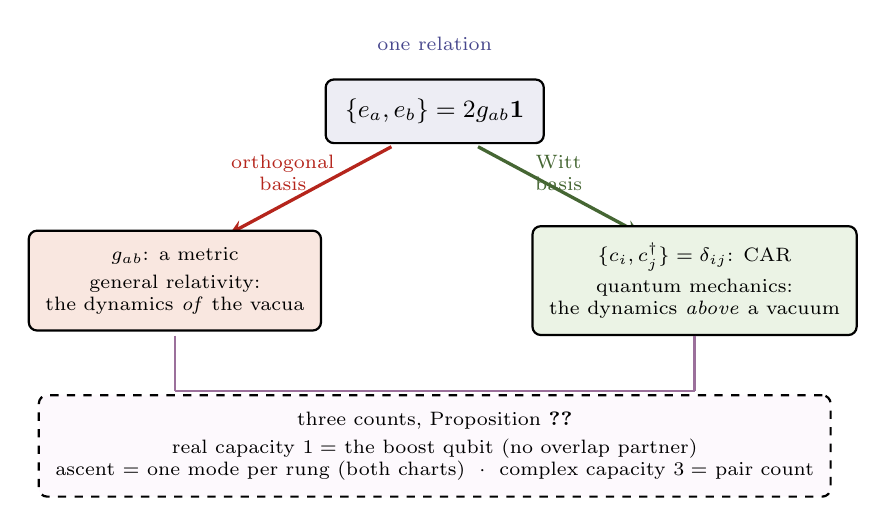
\begin{tikzpicture}[scale=1.0, >=stealth]
% the one relation at the top
\node[draw, thick, rounded corners=3pt, fill=MidnightBlue!8,
      font=\small, inner sep=7pt] (rel) at (0,2.5)
  {$\{e_{a}, e_{b}\} = 2g_{ab}\mathbf{1}$};
\node[font=\scriptsize, MidnightBlue!80, anchor=south] at (0,3.15)
  {one relation};
% two arrows down
\draw[->, very thick, BrickRed] (-0.55,2.05) -- (-2.6,0.95);
\node[BrickRed, font=\scriptsize, anchor=east, align=center] at (-1.15,1.72)
  {orthogonal\\basis};
\draw[->, very thick, OliveGreen!70!black] (0.55,2.05) -- (2.6,0.95);
\node[OliveGreen!70!black, font=\scriptsize, anchor=west, align=center]
  at (1.15,1.72) {Witt\\basis};
% left box: the metric
\node[draw, thick, rounded corners=3pt, fill=BrickRed!8, font=\scriptsize,
      align=center, inner sep=6pt] (geo) at (-3.3,0.35)
  {$g_{ab}$: a metric\\[2pt] general relativity:\\ the dynamics \emph{of} the vacua};
% right box: the CAR
\node[draw, thick, rounded corners=3pt, fill=OliveGreen!8, font=\scriptsize,
      align=center, inner sep=6pt] (car) at (3.3,0.35)
  {$\{c_{i}, c_{j}^{\dagger}\} = \delta_{ij}$: CAR\\[2pt] quantum mechanics:\\ the dynamics \emph{above} a vacuum};
% the three-counts bar
\node[draw, dashed, thick, rounded corners=3pt, fill=Plum!6,
      font=\scriptsize, align=center, inner sep=6pt] (ov) at (0,-1.75)
  {three counts, Proposition \ref{prop:capacity}\\[2pt]
   real capacity $1 =$ the boost qubit (no overlap partner)\\
   ascent $=$ one mode per rung (both charts) $\;\cdot\;$ complex capacity $3 =$ pair count};
\draw[Plum!70!black, thick] (-3.3,-0.35) -- (-3.3,-1.05);
\draw[Plum!70!black, thick] (3.3,-0.35) -- (3.3,-1.05);
\draw[Plum!70!black, thick] (-3.3,-1.05) -- (3.3,-1.05);
\end{tikzpicture}
\caption{The paper in one picture. The Clifford relation, read on an orthogonal basis, displays a metric and yields general relativity as the dynamics of how the vacuum varies from point to point; read on a Witt basis, the same relation is the canonical anticommutation relations and yields quantum mechanics as the dynamics of excitations above a vacuum chosen on a point's incidence line (Propositions \ref{prop:twopresentations} and \ref{prop:vacuummanifold}). Because the two readings are charts on one object rather than two objects, a count that both charts can perform is the same count on either; the boost qubit is a Witt-side count with no overlap partner and is drawn as such. The dashed bar lists three counts of Proposition \ref{prop:capacity}, real and complex, and says which is which: the real capacity of $(1,3)$, the boost qubit (clause (1), a single Witt-side count, not an overlap instance); the rung increment, one mode in either count (clause (2)), which is instance (i) of Proposition \ref{prop:overlap} and the input of its reading (iii); and the complex capacity three of the ascended space, the pair count (clause (3)), instance (ii).}
\label{fig:twocharts}
\end{figure}

Figure \ref{fig:twocharts} draws the thesis before the counts are stated.

\begin{proposition}[The two capacities, and three consequences]\label{prop:capacity}
Let $(V,Q)$ be real, nondegenerate, of signature $(p,q)$, $d = p+q$. The quantum presentation of Proposition \ref{prop:twopresentations} supports two mode counts, which differ in general and must not be conflated:
\[
r_{\R}(p,q) = \min(p,q), \qquad r_{\C}(p,q) = \lfloor d/2 \rfloor,
\]
the \emph{real capacity}, the number of modes realisable by real null vectors (Fact \ref{fact:capacity}), and the \emph{complex capacity}, the maximal isotropic dimension of $V_{\C}$, the number of modes of the complexified reading. They agree exactly when $|p - q| \leq 1$, in particular on the split signatures $(k,k)$; for $(1,3)$ they are $1$ and $2$, for $(2,4)$ they are $2$ and $3$. Three consequences, each labelled with the capacity it uses.
\begin{enumerate}
\item \emph{(The boost qubit; real.)} $r_{\R}(1,3) = 1$: Lorentzian signature has one real hyperbolic plane, unique up to an isometry of the whole space (all such planes are conjugate under $O(1,3)$), and the anisotropic complement is definite, so pre-ascent spacetime natively supports exactly one \emph{real} quantum mode, the boost qubit. The complex capacity is two, which is the Dirac spinor of $\Cl(1,3)_{\C}$ as a two-mode Fock space of dimension $2^{2} = 4$. This clause counts the modes of $(1,3)$ and says nothing about the single-mode thermality theorem, whose mode is the ladder pair of the ascent and is counted by neither $r_{\R}(1,3)$ nor $r_{\C}(1,3)$; what is said about that theorem is a reading, Proposition \ref{prop:overlap}(iii).
\item \emph{(Transport is capacity increment; both capacities.)} Each $(1,1)$ ascent adjoins one hyperbolic plane, hence one real null pair, hence one mode in either count: $r_{\R}$ and $r_{\C}$ each rise by exactly one per rung. The transport principle is capacity increment, and the tower's one-qubit-per-rung ladder (Fact \ref{fact:completion}) is its restatement.
\item \emph{(The ascended capacity is three; complex.)} $r_{\C}(2,4) = 3$: the complexified ascended $\C^{6}$ has maximal isotropic dimension three, which is the Standard-Model paper's pair count $(n+2)/2$ at spacetime dimension $n = 4$, the ambient signature being $(2,n)$, so that $d = n + 2$ and, for $n$ even, $\lfloor d/2 \rfloor = (n+2)/2$ \cite[Lem.~2.12]{ButlerT12}. Under that count the Standard-Model paper selects the strong force and four dimensions, on the two conditionalities it declares \cite[Prop.~4.3]{ButlerT12}. The real capacity of the ascended space is two: its third pair lies in the complexification, as the dark-matter paper's flag Fact records \cite[Fact~2.9]{ButlerT14}.
\end{enumerate}
Which capacity a physical count uses is therefore a statement to be made each time, not a residue: (1) is real, (3) is complex, (2) holds for both capacities. The successor problem is which of the two the state of Section \ref{sec:vacua} selects.
\end{proposition}

\begin{proof}
The real count is Fact \ref{fact:capacity}. For the complex count: a totally isotropic $U \subset V_{\C}$ satisfies $U \subseteq U^{\perp}$, and nondegeneracy gives $\dim U + \dim U^{\perp} = d$, so $2\dim U \leq d$; the bound is attained by the null spans of $\lfloor d/2 \rfloor$ pairs, built from the real hyperbolic planes together with pairs $(e + ie')/2$, $-(e - ie')/2$ on each two-dimensional block of the anisotropic kernel, whose square $\{c(e+ie'), c(e+ie')\} = 2(Q(e) - Q(e')) = 0$ vanishes because the kernel is definite and its diagonal entries equal. Both counts are exhibited by the script on $(1,1)$, $(1,3)$, $(2,4)$: the pairs are written down and every anticommutator computed. (1) $\min(1,3) = 1$; the anisotropic complement of the boost plane is the negative-definite $(e_{2}, e_{3})$ block, on which the script confirms $Q(ae_{2} + be_{3}) = -(a^{2} + b^{2}) < 0$ for rational $(a,b) \neq 0$, so no null vector lies in the anisotropic complement and no second anticommuting real pair exists; the Witt decomposition is unique up to isometry by Witt's extension theorem (Fact \ref{fact:witt}), which is the sense in which the boost plane is unique, and the same Witt fact is the uniqueness of the invariant ratio (Lemma \ref{lem:speed}(ii)). The agreement locus: for $p \leq q$, $r_{\R} = p$ and $r_{\C} = \lfloor d/2 \rfloor = \lfloor (p+q)/2 \rfloor$, so $r_{\R} = r_{\C}$ if and only if $2p \leq p + q \leq 2p + 1$, that is $0 \leq q - p \leq 1$, and symmetrically for $q \leq p$; the script's grid check illustrates this. (2) $\min(p+1,q+1) = \min(p,q) + 1$ and $\lfloor (d+2)/2 \rfloor = \lfloor d/2 \rfloor + 1$, arithmetic identities, recorded by the script on the grid $p, q \leq 8$. (3) $\lfloor 6/2 \rfloor = 3$ and $\min(2,4) = 2$, with the three pairs of $\Cl(2,4)_{\C}$ exhibited, two real and one complex.
\end{proof}

\section{Spacetime as the manifold of vacuum lines}\label{sec:vacua}

\begin{proposition}[Spacetime as the manifold of vacuum lines]\label{prop:vacuummanifold}
Four clauses.
\begin{enumerate}
\item \emph{(Every point is null.)} Under the embedding of Fact \ref{fact:purespinor}, $\ip{X(x)}{X(x)} = 0$ identically: every point of spacetime is a non-invertible element of the algebra. Division by zero is not confined to special loci but is the condition of every point. The embedding needs $Q(x) = c^{2}t^{2} - |\mathbf{x}|^{2}$ dimensionally homogeneous, so the null embedding is where the third constant first enters the series (Lemma \ref{lem:speed}).
\item \emph{(Every point is a projective line of vacua.)} The point's null vector acts on the Fock module of Fact \ref{fact:purespinor} as a nilpotent, $c(X(x))^{2} = \ip{X(x)}{X(x)} = 0$, whose kernel has dimension four on the eight-dimensional module and exactly two on the twistor half $\T$: that two-dimensional kernel is the point's incidence line $L_{x}$. Every twistor $u$ on $L_{x}$ is the Fock vacuum of its own three-pair system $W_{u}$, and $X(x) \in W_{u}$ for each of them: a point is not one vacuum but a projective line of distinct vacua, all of whose isotropic systems contain its null vector. Complexified compactified spacetime is the manifold of such lines, the Klein quadric of lines in $\mathbb{P}(\T)$, of which the real compactified spacetime is the real slice (double covered by the completion's fibre quadric, Fact \ref{fact:purespinor}); it is not the pure-spinor variety $\mathbb{P}(\T)$, which has one dimension fewer. Two points are null-separated exactly when their incidence lines share a vacuum: $\ip{X(x)}{X(y)} = -\tfrac12 Q(x - y)$.
\item \emph{(The location of each theory.)} The two theories then read: general relativity is the dynamics \emph{of} the vacua, how the vacuum family varies from point to point, carried by the connection; quantum mechanics is the dynamics \emph{above} a vacuum, excitations over a chosen vacuum obeying the CAR of Proposition \ref{prop:twopresentations}. The choice of a vacuum on a point's incidence line is an extra datum, a null direction at the point, which the reading must supply and the point does not.
\item \emph{(Ubiquity, and what a singularity is.)} Quantum mechanics holds everywhere because every point carries its incidence line of vacua; a singularity is where the vacuum family degenerates, where the choice of vacuum itself becomes operator-valued, which is the sheaf paper's localisation theorem, in the Schwarzschild form the singularity paper carries, read in this language \cite[Thm.~4.4, Cor.~4.5, Thm.~8.12]{ButlerT4}, \cite[App.~B]{ButlerT5}.
\end{enumerate}
The series' statement is thereby sharpened: division by zero does not only mark special loci, it constitutes every point.
\end{proposition}

\begin{proof}
(1) is the nullity computation of Fact \ref{fact:purespinor}. The script re-verifies it on the flat model with the inner product computed, not assumed: with $n_{0} = (e_{+} + e_{-})/2$, $n_{\infty} = e_{+} - e_{-}$ for $e_{\pm}^{2} = \pm 1$, it confirms $n_{0}^{2} = n_{\infty}^{2} = 0$, $\ip{n_{0}}{n_{\infty}} = 1$, then for six rational points with $Q(x)$ timelike, null and spacelike computes $\ip{X(x)}{X(x)} = 0$ and $X(x)^{2} = 0$ in the algebra with $X(x) \neq 0$, and confirms that any other slot coefficient $c$ gives $\ip{X}{X} = Q(x)(1 + 2c) \neq 0$. A nonzero nilpotent is not invertible. (2) By Fact \ref{fact:purespinor} a nonzero twistor $u$ has $\dim W_{u} = 3$ and $W_{u}$ determines $[u]$; and $c(X)u = 0$ if and only if $X \in W_{u}$, by the definition of $W_{u}$. So the twistors annihilated by $c(X(x))$ are exactly those whose isotropic system contains $X(x)$, and the set of such $[u]$ is the incidence line of the chart theorem, the line of $\mathbb{P}(\T)$ that the simple bivector $X(x)$ represents. The kernel dimensions follow from nilpotency and the module structure: on the eight-dimensional Fock module a nonzero null vector has kernel of dimension exactly four, because the nonzero null vectors form a single $O(6,\C)$-orbit (Witt's extension theorem, Fact \ref{fact:witt}), $c$ is equivariant under the Pin lift, so the rank of $c(X)$ is constant on the orbit, and at $X = w_{1}$ the operator is the wedge with one basis element of $W$, which annihilates exactly the four monomials containing it; and $c(X)$ swaps the chirality halves, so its kernel splits as two plus two. The script builds the Fock model explicitly (wedge and contraction on $\Lambda^{\bullet}W$, $\dim 8$, with the six ambient generators realised and all thirty-six anticommutators checked), and for each of the six points computes: $c(X)^{2} = 0$; kernel of dimension four, and two on each half; that two independent twistors on the line and their sum each have a three-dimensional annihilator, pairwise distinct; that $X(x)$ lies in each of those annihilators; and, across the fifteen pairs of points, that the lines are pairwise distinct and meet exactly when the points are null-separated. The null-separation criterion in general: expanding with $n_{0}^{2} = n_{\infty}^{2} = 0$ and $\ip{n_{0}}{n_{\infty}} = 1$ gives $\ip{X(x)}{X(y)} = \ip{x}{y} - \tfrac12 Q(x) - \tfrac12 Q(y) = -\tfrac12 Q(x-y)$, which the script confirms on all fifteen pairs; and two incidence lines share a vacuum $u$ if and only if $X(x), X(y) \in W_{u}$ for some $u$, if and only if $X(x)$ and $X(y)$ span a totally isotropic plane (any two vectors of a maximal isotropic subspace are orthogonal; conversely an isotropic plane of $\C^{6}$ lies in exactly two maximal isotropic subspaces, which meet in it, so their intersection has odd codimension one in each and they lie in opposite families, exactly one of them the annihilator of a twistor in $\T$, which is also why two meeting incidence lines meet in one point), if and only if $\ip{X(x)}{X(y)} = 0$, since both are null. (3) and (4) are readings of (1)-(2) together with the imported theorems named, and are stated at that level: the content is the placement of the two theories on one object, not a new dynamical claim.
\end{proof}

\paragraph{The connection in words.} Gravity enters when the same construction is made at every point. The relation holds everywhere, so every point has its own light rays, its own bivector $\sigma$, and its own mode. That raises a question the relation cannot answer on its own: given the mode here, which mode over there is the same one? The connection answers it by carrying $\sigma$ from one point to the next along a path, keeping it as unchanged as the geometry allows, and this is what clause (3) means by the dynamics of the vacua. The answer can depend on the path. Carry $\sigma$ from here to there by one route and back by another, and it need not come home as the $\sigma$ you started with; it comes back tilted. That tilt is curvature, and the tilt is gravity (Figure \ref{fig:holonomy}).

Two things should not be confused with this. The sign choice, which of the two rays is the creation operator, is not what tilts: a yes-or-no choice carried round a loop comes back either the same or flipped, and in a connected orientable spacetime it comes back the same. What tilts is the plane the choice was made on. And the fact that $g_{ab}$ takes different values at different points is not by itself curvature either: flat space can be written in coordinates where $g_{ab}$ varies and the light cones lean over, and nothing tilts on return. Curvature is what happens round the loop, not what the components look like at a point. Nothing here says why the geometry tilts things the way it does: the relation is satisfied by any metric, and what picks one is the field equation, which the geometry paper supplies \cite[Thm.~4.5]{ButlerT6} and this one does not. Gravity is not something added to the modes; it is the fact that the modes at different points cannot all be made the same mode, and the one bivector $\sigma$ is at once the label that says which state is occupied, the boost in its plane, and the thing that comes back tilted.

\begin{figure}[ht]
\centering
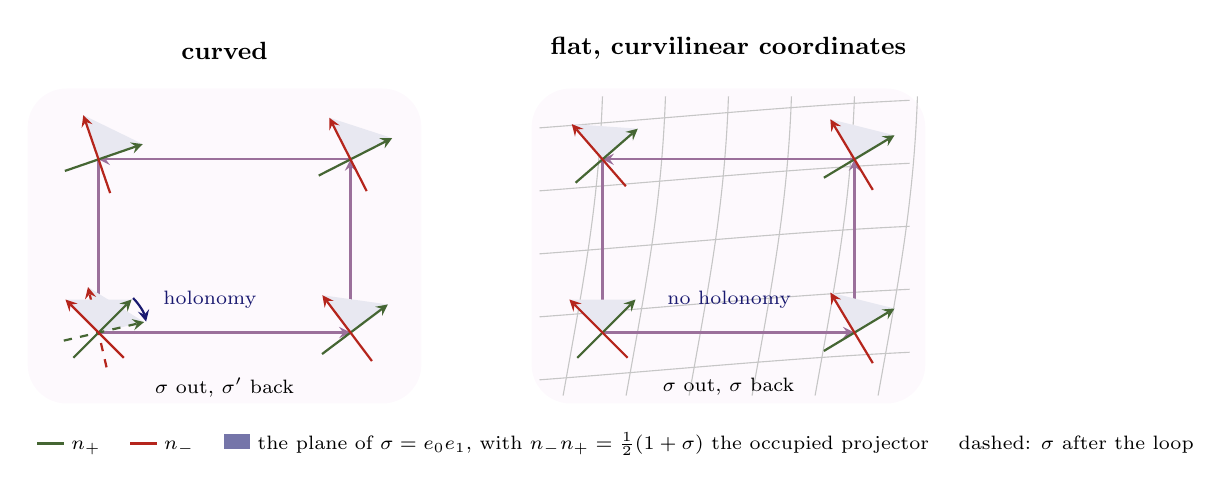
\begin{tikzpicture}[scale=1.0, >=stealth]
% ---------------- left panel: curved ----------------
\begin{scope}[shift={(0,0)}]
  \node[font=\small\bfseries, anchor=south] at (1.6,3.35) {curved};
  \fill[Plum!6, rounded corners=14pt] (-0.9,-0.9) rectangle (4.1,3.1);
  \draw[Plum!70!black, thick, ->] (0,0) -- (3.2,0);
  \draw[Plum!70!black, thick, ->] (3.2,0) -- (3.2,2.2);
  \draw[Plum!70!black, thick, ->] (3.2,2.2) -- (0,2.2);
  \draw[Plum!70!black, thick, ->] (0,2.2) -- (0,0.05);
  \cone{3.2,0}{-8}{}
  \cone{3.2,2.2}{-18}{}
  \cone{0,2.2}{-26}{}
  \cone{0,0}{-32}{dashed}
  \cone{0,0}{0}{}
  \draw[MidnightBlue, thick, ->] (45:0.62) arc (45:13:0.62);
  \node[MidnightBlue, font=\scriptsize, anchor=west] at (0.7,0.42) {holonomy};
  \node[font=\scriptsize, anchor=north] at (1.6,-0.45) {$\sigma$ out, $\sigma'$ back};
\end{scope}
% ---------------- right panel: flat, curvilinear coordinates ----------------
\begin{scope}[shift={(6.4,0)}]
  \node[font=\small\bfseries, anchor=south] at (1.6,3.35) {flat, curvilinear coordinates};
  \fill[Plum!6, rounded corners=14pt] (-0.9,-0.9) rectangle (4.1,3.1);
  \foreach \x in {-0.5,0.3,1.1,1.9,2.7,3.5} {
    \draw[gray!45, thin] (\x,-0.8) .. controls (\x+0.25,0.6) and (\x+0.45,1.6) .. (\x+0.5,3.0);
  }
  \foreach \y in {-0.6,0.2,1.0,1.8,2.6} {
    \draw[gray!45, thin] (-0.8,\y) .. controls (0.8,\y+0.12) and (2.4,\y+0.28) .. (3.9,\y+0.35);
  }
  \draw[Plum!70!black, thick, ->] (0,0) -- (3.2,0);
  \draw[Plum!70!black, thick, ->] (3.2,0) -- (3.2,2.2);
  \draw[Plum!70!black, thick, ->] (3.2,2.2) -- (0,2.2);
  \draw[Plum!70!black, thick, ->] (0,2.2) -- (0,0.05);
  \cone{3.2,0}{-14}{}
  \cone{3.2,2.2}{-14}{}
  \cone{0,2.2}{-4}{}
  \cone{0,0}{0}{}
  \node[font=\scriptsize, anchor=north] at (1.6,-0.45) {$\sigma$ out, $\sigma$ back};
  \node[MidnightBlue, font=\scriptsize, anchor=west] at (0.7,0.42) {no holonomy};
\end{scope}
% ---------------- legend ----------------
\node[font=\scriptsize, align=left, anchor=north west] at (-0.9,-1.15)
  {\textcolor{OliveGreen!70!black}{\rule[0.5ex]{1.2em}{1pt}} $n_{+}$ \quad
   \textcolor{BrickRed}{\rule[0.5ex]{1.2em}{1pt}} $n_{-}$ \quad
   \textcolor{MidnightBlue!60}{\rule{1.2em}{0.7em}} the plane of $\sigma = e_{0}e_{1}$, with $n_{-}n_{+} = \tfrac12(1+\sigma)$ the occupied projector \quad
   dashed: $\sigma$ after the loop};
\end{tikzpicture}
\caption{What gravity does to the mode. At every point the relation supplies two light rays $n_{\pm} = \tfrac12(e_{0} \pm e_{1})$ in a timelike plane and the plane's unit bivector $\sigma = e_{0}e_{1}$, whose sign decides which ray is the creation operator ($n_{-}n_{+} = \tfrac12(1+\sigma)$ is the occupied projector). Left: on a curved patch the connection carries $\sigma$ round a closed loop and returns it as a different bivector of the same point, the frame having been rotated by the holonomy; that rotation is curvature, and it acts on the plane, not on the discrete sign, which comes back unchanged in any connected orientable spacetime. Right: on flat space in curvilinear coordinates the components $g_{ab}$ vary and the drawn cones lean with the coordinates, but the transported $\sigma$ comes back as itself; leaning cones are a coordinate description and not curvature. The figure illustrates Proposition \ref{prop:vacuummanifold}(3) and does not replace it.}
\label{fig:holonomy}
\end{figure}

\begin{proposition}[The overlap table, sorted]\label{prop:overlap}
Three numerical agreements in this series are read as consequences of the one relation having two charts. They are not of one kind, and the proposition sorts them; none is an agreement of independent computations. \emph{(i) One count in two vocabularies.} The tower's one-qubit-per-rung ladder is read off the periodicity isomorphism $\Cl(p+1,q+1) \cong \Mat(2, \Cl(p,q))$, one matrix doubling per rung; the capacity increment of Proposition \ref{prop:capacity}(2) is index arithmetic. The isomorphism is the tower paper's structure theorem (Fact \ref{fact:completion}); its dimension shadow $2^{p+q+2} = 4 \cdot 2^{p+q}$ and the increment are identities that cannot fail, and the step that reads a matrix doubling as one mode is exactly the identification of Proposition \ref{prop:twopresentations}; the content is that the metric reading's doubling and the Witt reading's mode are one count. \emph{(ii) An identification.} The pair count $(n+2)/2 = 3$ at spacetime dimension $n = 4$, under which the Standard-Model paper selects the strong force and four dimensions on its two declared conditionalities, is proved there to be the maximal isotropic dimension of the complexified ascended space, by the same argument this paper gives for the complex capacity \cite[Lem.~2.12]{ButlerT12}; its equality with $r_{\C}(2,4)$ of Proposition \ref{prop:capacity}(3) is therefore an identification and not an agreement: the twistor's pairs are the fermionic modes of the complex reading, so the Standard-Model paper's count is a quantum capacity, and what is new here is only the extension to arbitrary signature with the attainment construction. \emph{(iii) A reading.} The thermality theorem (Fact \ref{fact:thermality}) is single-mode, its mode being the ladder pair of the ascent, a mode adjoined by the rung and not the boost pair of $(1,3)$; Proposition \ref{prop:capacity}(2) says a rung adjoins exactly one mode in either count. That the theorem is single-mode \emph{because} one rung was ascended is the structural explanation this paper offers, and it is a reading of the two results together, not a computation; the theorem installs one mode per point of the singular boundary (Fact \ref{fact:thermality}, \cite[Thm.~8.12]{ButlerT4}), so the reading concerns each marginal and not a capacity ceiling. At observation level, each presentation also carries a constant, and the three constants are at three levels: $\hbar$ as the ordering shift of the Witt presentation, the half-per-mode shift proved in the twistor paper T9 \cite[Prop.~5.6]{ButlerT9}; $G$ as the compositeness scale of the metric presentation, the dimension-two irrelevance the dark-energy paper T10 reads at structural level from its acoustic no-go, the no-go itself conditional on the singularity paper's premise (Q), within an acoustic programme that paper closes at the mixed level of its inputs, the sphere step conditional on the indifference premise \cite[Prop.~5.2, Rem.~5.3, Assembly~5.5]{ButlerT10}; and $c$ as the datum of the transition between the two charts, invisible in the Witt chart, which contains rapidity and no other quantity, and fixed in the metric chart, which contains time and length separately (Lemma \ref{lem:speed}, proved). The third is placed by a different mechanism from the first two, and it is a conformal invariant, surviving every conformal step the first two do not. This is an identification of \emph{where} the constants enter, not a derivation of their values, and it remains the synthesis's weakest point, flagged as such; what can be said in its favour is this: $c$ has no value to derive, its number being a unit convention, and in the Planck system all three are, so a placement can be nothing more than this.
\end{proposition}

\begin{proof}
(i) is two identities and one identification: the script records on the grid $p, q \leq 6$ that $\dim \Cl(p+1,q+1) = 4\dim\Cl(p,q)$ while $r_{\R}$ and $r_{\C}$ each rise by one, arithmetic that cannot fail, and the identification is Proposition \ref{prop:twopresentations}, which makes the change of chart an isomorphism of the algebra rather than an analogy. (ii) is a lemma read across two papers, and its content is the identification stated, proved to no standard beyond its statement. (iii) is a reading and is labelled one. The constants clause is an identification for $\hbar$ and $G$, proved to no standard beyond its own statement, which is why it is flagged; the placement of $c$ is Lemma \ref{lem:speed}.
\end{proof}

\begin{remark}[Two residues, named so the synthesis can be refuted]\label{rem:synthesisresidues}
First, \emph{state selection}: Proposition \ref{prop:twopresentations} identifies the kinematic algebra, and the physical state remains the flagged remainder of the thermality theorem; a selected state incompatible with the incidence-line structure of Proposition \ref{prop:vacuummanifold}, or one requiring more than the two real or three complex modes that the single ascent the conformal completion licenses, to $\Cl(2,4)$, supplies (Fact \ref{fact:purespinor}, Proposition \ref{prop:capacity}), would break the vacuum-line reading. Second, \emph{the laboratory problem}: whether ordinary nonrelativistic quantum mechanics is recoverable as excitation dynamics above a vacuum chosen on a regular point's incidence line, with the Hamiltonian descending from the boost clock (the boost generator of the horizon pair, the singularity paper's clock) in the appropriate limit, is settled by no numbered result here; Proposition \ref{prop:vacuummanifold}(4) claims ubiquity only. Sections \ref{sec:lab}-\ref{sec:experience} carry that computation out at the levels they declare, and the claim is quantum mechanics everywhere, not only at interfaces. What the laboratory leaves as its remainder, after the sharpening of Lemmas \ref{lem:square} to \ref{lem:onedatum}, is not the form of the law, which is forced, but why the evolution parameter is the frame's time and which frame: the frame cannot be sourced from the law, since the frozen point is $SO(1,4)$-invariant and any theorem selecting a $\gamma_{0}$ would break that; it is state data or observer data, and sourcing it is thermal time plus state selection, the geometric modular action the capstone carries as the open problem together with successor (2) here, and it is named and not opened. A third item, at programme level: if the earliest correlations are sourced by the descent, the primordial spectrum is the shape-shadow of a fibre state projected through the freezing, a computation whose output would confront the measured spectral index and would be a further registered stance; it is named in the successors and assigned to the capstone \cite{ButlerT17}.
\end{remark}


\begin{lemma}[The third constant is the conversion constant between the charts]\label{lem:speed}
Let $(V, Q)$ be a real quadratic space of signature $(p, q)$, $n = p + q \geq 2$, with events carrying a time coordinate and space coordinates measured in independently chosen units, so that a quadratic form on events is dimensionally homogeneous only after a conversion constant $c$ is chosen, $Q = c^{2}t^{2} - |\mathbf{x}|^{2}$ in the Lorentzian case. Then:
\begin{enumerate}
\item[(i)] \emph{(Existence and finiteness.)} A finite invariant ratio of length to time exists if and only if $Q$ is nondegenerate and mixed, $pq \neq 0$: the null cone is that invariant ratio, preserved by every isometry, and it is nonempty exactly when the signature is mixed; dividing $Q$ by $c^{2}$ and letting $c \to \infty$ degenerates $Q$ to the rank-one form $t^{2}$, whose zero set is the simultaneity hyperplane, the Galilean case the root paper sets aside. The word \emph{speed} is reserved for the case of clause (iv). Two of the three standing hypotheses of the root paper's no-go theorem \cite[Thm.~4.2]{ButlerT1}, nondegenerate and mixed, are jointly the existence of a finite invariant ratio; the third, $n \geq 3$, is not needed here and enters only through Zeeman's theorem below.
\item[(ii)] \emph{(One number.)} The invariant ratio is a property of a hyperbolic plane, and the isometry group is transitive on the hyperbolic planes of $(V, Q)$ (Witt's extension theorem, Fact \ref{fact:witt}), so every hyperbolic plane carries the same $c$. This is the Witt fact of Proposition \ref{prop:capacity}(1): the uniqueness of the boost qubit and the uniqueness of the invariant ratio are one statement.
\item[(iii)] \emph{(Invisible in the Witt chart, fixed in the metric chart.)} On a hyperbolic plane with orthonormal pair $e_{0}, e_{1}$, $e_{0}^{2} = 1$, $e_{1}^{2} = -1$, the Witt chart $f_{\pm} = \tfrac12(e_{0} \pm e_{1})$, $f_{+} \cdot f_{-} = \tfrac12$, has a one-parameter freedom the metric chart does not show, $f_{+} \to \lambda f_{+}$, $f_{-} \to f_{-}/\lambda$, $\lambda > 0$; that rescaling is exactly the boost rotor of rapidity $\eta = \log\lambda$ acting on the orthonormal frame, $R = \cosh(\eta/2) - \sinh(\eta/2)\,e_{0}e_{1}$, with $R e_{0}\tilde{R} = \cosh\eta\, e_{0} + \sinh\eta\, e_{1}$ and $R f_{+}\tilde{R} = e^{\eta}f_{+}$, and the coordinate velocity of the boosted time axis is $c\tanh\eta$. The Witt chart contains rapidity, a dimensionless number, and no other quantity; the metric chart contains time and length separately; the transition from one to the other is what requires the conversion constant $c$. That the algebra fixes orbits and not speeds, as the entropy paper states \cite[Fact~2.2]{ButlerT8}, is this clause: the Witt chart is scale-free, and the geometric normalisation that converts rapidity to time is the chart transition.
\item[(iv)] \emph{(A speed with an arrow.)} The set $\{Q > 0\}$ retracts onto the unit sphere of the positive part and has the components of $S^{p-1}$: two when $p = 1$, one when $p \geq 2$, none when $p = 0$; symmetrically $\{Q < 0\}$ splits exactly when $q = 1$. Hence a nondegenerate form admits a future/past split, a $\mathbb{Z}_{2}$ of time orientation, if and only if $\min(p, q) = 1$. The dark-matter paper's causal criterion \cite[Prop.~3.1]{ButlerT14}, stated there as a definition, is thereby a theorem about the cone: a signature has a single time if and only if its timelike set is disconnected. $c$ is a speed, a length over one time, precisely in the causal signatures; in $(2,2)$ the null cone exists and determines the form, so an invariant ratio exists, but there is no single time to divide by and no arrow, and the invariant is not a speed.
\end{enumerate}
With Fact \ref{fact:cone}, the cone determines $Q$ up to scale, so $c$ is a conformal invariant and survives every conformal step of the series, the projective-to-conformal completion, the twistor correspondence and the tractor bundle, which is why those papers can set $c = 1$ with no effect on their results; $G$ does not survive the conformal step, needing the scale the conformal class forgets, and $\hbar$ does not survive the classical chart, needing the ordering. The three constants therefore sit at three levels: $c$ at the conformal level (the cone), $G$ at the metric level (the scale), $\hbar$ at the Witt level (the ordering); and the exponent matrix of $(c, \hbar, G)$ over (length, time, mass) has determinant $-2$, so the three together fix the three base units and every remaining constant is dimensionless over (length, time, mass), while $\hbar$ and $G$ alone fix no base unit. Zeeman's theorem (Fact \ref{fact:cone}) connects (iv) back to the conformal level: in a causal signature with $n \geq 3$ the causal automorphisms are the conformal ones up to dilation.
\end{lemma}

\begin{proof}
(i) The null cone is $\{Q = 0\}$, preserved by isometries by definition; it contains a nonzero vector iff $pq \neq 0$ (the root paper's null-locus criterion, Fact \ref{fact:cone}); the script checks that $Q/c^{2} = \mathrm{diag}(1, -c^{-2}, -c^{-2}, -c^{-2})$ has signature $(1,3)$ at $c = 1, 10, 1000$ and that at $c = \infty$ the form is $\mathrm{diag}(1, 0, 0, 0)$, of rank one with radical the simultaneity hyperplane. (ii) is Witt's extension theorem (Fact \ref{fact:witt}), which the dark-matter paper imports and Proposition \ref{prop:capacity} uses: two hyperbolic planes are isometric, so the isometry between them extends to an isometry of $(V, Q)$. The script takes three rational null pairs of $(1,3)$, $n \cdot m = -1$, spanning three pairwise distinct hyperbolic planes, and computes that their anisotropic complements all have signature $(0,2)$, the witness the theorem needs; the theorem itself is imported. (iii) The rotor identities are computed exactly in $\Cl(1,1)$ at $\lambda = e^{\eta} = 4$, $\cosh\eta = \tfrac{17}{8}$, $\sinh\eta = \tfrac{15}{8}$: $R\tilde{R} = 1$, $Re_{0}\tilde{R} = \cosh\eta\,e_{0} + \sinh\eta\,e_{1}$ with norms preserved, $Rf_{\pm}\tilde{R} = \lambda^{\pm 1}f_{\pm}$, the null lines the fixed lines of every boost, and the velocity $\tanh\eta = (\lambda^{2} - 1)/(\lambda^{2} + 1) = \tfrac{15}{17}$; the sign convention matters, the opposite sign in the rotor reversing the boost, and the script fixes it as stated. (iv) The retraction $(a, b) \mapsto (a, tb)$, $t \in [0, 1]$, on $\{Q > 0\}$ written as $|a|^{2} - |b|^{2} > 0$ in an orthonormal basis, deformation-retracts it onto $\{|a| = 1, b = 0\} \cong S^{p-1}$; $S^{0}$ has two components, $S^{k}$ for $k \geq 1$ one, and $S^{-1}$ is empty. The script checks the component counts on sample points: on the signatures $(1,0)$ to $(3,2)$ and $(0,3)$ it counts the classes of a union-find over rational sample points of $\{Q > 0\}$ joined by exact segments with certified $Q$-minima, compares the count with the $S^{p-1}$ count entered as a literal, certifies two classes as distinct by the sign of the time coordinate, and checks the disjunction against $\min(p, q) = 1$ on seven signatures up to $n = 5$; the proof of the count is the retraction above, not the script; the cone-determines-form clause of Fact \ref{fact:cone} is also checked, on the signatures up to $(3,3)$, as the one-dimensionality of the space of symmetric forms vanishing on the rational null vectors. The exponent determinant is arithmetic the script performs, together with the statement that no monomial in $\hbar$ and $G$ alone has the dimension of a length, a time, or a mass. Nothing here derives a value for $c$: its number is a unit convention, and in the Planck system all three are; the only derivable things are dimensionless ratios, which the capstone examines.
\end{proof}

\begin{remark}[Where exhaustiveness first fails: the $\nu = 4$ quadric]\label{rem:quadric}
Fact \ref{fact:purespinor}'s statement that every twistor is a vacuum is Cartan's purity theorem at $2\nu = 6$ (Fact \ref{fact:cartan}), and it is a low-dimensional coincidence: the even sector of $\nu$ modes has projective dimension $2^{\nu - 1} - 1$ and the vacua form the spinor variety of dimension $\nu(\nu - 1)/2$, which agree at $\nu = 1, 2, 3$ and first differ at $\nu = 4$, seven against six. At $\nu = 3$ the vacuum orbit is open in the even sector and is everything: this is the transitivity of $SL(4, \C)$ on $\mathbb{P}^{3}$, the exceptional isomorphism $\mathrm{Spin}(6, \C) \cong SL(4, \C)$ on which the twistor correspondence rests, so the reason every twistor is a vacuum is the reason twistor space is a $\mathbb{P}^{3}$ on which the conformal group acts transitively. At $\nu = 4$, writing an even state as $\psi = \psi_{0}|0\rangle + \sum_{i<j}\psi_{ij}|ij\rangle + \psi_{1234}|1234\rangle$, the vacuum condition is the single quadric
\[
\mathcal{Q}(\psi) \;=\; \psi_{0}\,\psi_{1234} \;-\; \bigl(\psi_{12}\psi_{34} - \psi_{13}\psi_{24} + \psi_{14}\psi_{23}\bigr) \;=\; 0 ,
\]
the $\mathrm{Spin}(8)$-invariant triality form, and the reason is the Thouless form of Fact \ref{fact:cartan}:
\[
\exp\Bigl(\sum_{i<j} A_{ij}a^{\dagger}_{i}a^{\dagger}_{j}\Bigr)|0\rangle \;=\; |0\rangle + \sum_{i<j} A_{ij}|ij\rangle + \mathrm{Pf}(A)|1234\rangle
\]
exactly, so the quartic coefficient of a vacuum is forced to be the Pfaffian of its quadratic coefficients, and at $\nu = 3$ there is no quartic term to constrain. The script verifies the identity on random antisymmetric $A$, the criterion $\mathcal{Q} = 0$ against the Gaussian purity test $M^{2} = -1$ on random even states, the tangent ranks $1 + \nu(\nu - 1)/2$ of the vacuum orbit at $\nu = 2, 3, 4$ with the orbit open at $\nu = 3$ and a hypersurface at $\nu = 4$, and a non-vacuum's orbit rank $8$. What this says for this paper: the incidence-line structure of Proposition \ref{prop:vacuummanifold} is a complex-capacity statement at $\nu = 3$, where purity is automatic, while the real capacity of $(1,3)$, one, admits no pairing at all ($\nu(\nu - 1)/2 = 0$); that answers half of successor problem (1). The definition of entanglement as mismatch between Witt decompositions, which the singularity paper's boundary mode space and its thermofield angle $\tan^{2}\theta = e^{-\omega/T}$ both use \cite[Lem.~7.2, Thm.~7.3]{ButlerT5}, is exhaustive at $\nu \leq 3$ and stops being so at $\nu = 4$, where $\mathcal{Q}$ is the order parameter of the states that belong to no Witt decomposition; that is the first instance of the quasi-free limit of the series' state class, named here and not opened.
\end{remark}

\section{The laboratory: the slow shadow}\label{sec:lab}

The synthesis does not by itself reach the laboratory. Nonrelativistic quantum mechanics postulates three things the framework must either source or concede: a preferred time split, an imaginary unit, and a mass term. Of these the section sources one outright (the mass, at the level its Fact holds), sources half of the first (the time orientation, under the Standard-Model paper's Hypothesis (S)), declares the other half of the first, the rest frame, unsourced, and proves that the second was not a separate postulate at all: given the law, the imaginary unit is the rest frame read through it (Lemma \ref{lem:onedatum}). It begins with the statement that is proved outright, and returns after the descent to the three lemmas that sharpen it.

\begin{lemma}[The vector derivative is the covariant first-order operator]\label{lem:vectorderivative}
Let $D = A^{\mu}\partial_{\mu}$ be a first-order operator with constant coefficients $A^{\mu} \in \Cl(1,3)$ acting by left multiplication on $\Cl(1,3)$-valued fields on Minkowski space (hence on every minimal left ideal), and suppose $D$ is covariant under the spin group: $D(R\,\psi\circ\Lambda_{R}^{-1}) = R\,(D\psi)\circ\Lambda_{R}^{-1}$ for every rotor $R \in \mathrm{Spin}^{+}(1,3)$, $\Lambda_{R}$ its vector transformation. Then $A^{\mu} = \gamma^{\mu}(a + bI)$ for real $a, b$, with $I = \gamma_{0}\gamma_{1}\gamma_{2}\gamma_{3}$ the pseudoscalar: $D = (a - bI)\nabla$ for the vector derivative $\nabla = \gamma^{\mu}\partial_{\mu}$, and $a - bI$ is invertible whenever $(a,b) \neq (0,0)$. Among covariant constant-coefficient first-order operators acting by left multiplication, the vector derivative is unique up to an invertible constant factor. (Right multiplications are outside the class: $\psi \mapsto \nabla\psi\,B$ for constant $B$ is covariant, and is not of the form $A^{\mu}\partial_{\mu}$ acting on the left unless $B$ is central.)
\end{lemma}

\begin{proof}
Writing out the covariance condition on $\psi \circ \Lambda_{R}^{-1}$ and cancelling the field, it is equivalent to $R^{-1}A^{\mu}R = M(R)^{\mu}{}_{\nu}A^{\nu}$ for every rotor, where $M(R)$ is the vector matrix defined by $R^{-1}\gamma^{\mu}R = M(R)^{\mu}{}_{\nu}\gamma^{\nu}$. This is a linear condition on the $64$-dimensional space of quadruples $(A^{0}, \dots, A^{3})$. Two solutions are known: $A^{\mu} = \gamma^{\mu}$, by the definition of $M(R)$; and $A^{\mu} = \gamma^{\mu}I$, because $I$ commutes with every even element, so $R^{-1}\gamma^{\mu}IR = R^{-1}\gamma^{\mu}R\,I$. For the converse it suffices to show that finitely many rotors already cut the solution space down to the span of these two, since the space of solutions for all rotors is contained in the space of solutions for any subset. The script imposes the condition for six rational rotors, the boosts $\tfrac54 + \tfrac34\gamma_{0}\gamma_{1}$, $\tfrac{13}{12} + \tfrac{5}{12}\gamma_{0}\gamma_{2}$, $\tfrac{17}{15} + \tfrac{8}{15}\gamma_{0}\gamma_{3}$ and the rotations $\tfrac35 + \tfrac45\gamma_{1}\gamma_{2}$, $\tfrac{5}{13} + \tfrac{12}{13}\gamma_{1}\gamma_{3}$, $\tfrac{8}{17} + \tfrac{15}{17}\gamma_{2}\gamma_{3}$ (each of unit norm, $R\tilde{R} = 1$, exactly), and computes the kernel of the stacked $384 \times 64$ system over the Gaussian rationals: it is two-dimensional and contains the two known solutions, so it equals their span. Finally $\gamma^{\mu}(a + bI) = (a - bI)\gamma^{\mu}$ because $I$ anticommutes with vectors, and $(a - bI)(a + bI) = a^{2} + b^{2}$ because $I^{2} = -1$ in $\Cl(1,3)$; the script checks the anticommutation on all four generators, the identity $\gamma^{\mu}(a+bI) = (a-bI)\gamma^{\mu}$ on instances, and the norm identity.
\end{proof}

\begin{proposition}[Schr\"odinger as the slow shadow]\label{prop:slowshadow}
The laboratory equation is the algebra's own first-order operator viewed from inside a rest frame. The chain, in four steps, with each input's provenance declared.
\begin{enumerate}
\item \emph{(The operator; proved.)} The first-order operator is the vector derivative $\nabla = \gamma^{\mu}\partial_{\mu}$, unique up to an invertible constant factor among covariant constant-coefficient first-order operators acting by left multiplication (Lemma \ref{lem:vectorderivative}): native to the Clifford presentation, no postulate.
\item \emph{(The mass comes from the condensate; sourced. The form of the law; forced, given first order.)} The equation of motion is the Dirac-Hestenes equation $\nabla\psi\, I\sigma_{3} = m\,\psi\gamma_{0}$, Hestenes' real form of the Dirac equation \cite{Hestenes1967, Hestenes1975}. What is imported is one sentence, that the law is first order, Dirac's factorisation of the mass shell; the form is then forced: a first-order covariant law $\nabla\psi = m\psi C$ with constant right factor squares to Klein-Gordon at mass $m$ iff $C^{2} = -1$ (Lemma \ref{lem:square}), and every odd such $C$ is the Dirac-Hestenes factor up to the representation freedom and a constant chiral phase, the latter a field redefinition for the single free minimally coupled fermion treated here (Lemma \ref{lem:oddroots}). Its mass parameter is the mass of Fact \ref{fact:condensate}: applying $\nabla$ twice gives $\nabla^{2}\psi = -m^{2}\psi$, so every component of a solution is a Klein-Gordon field $(\Box + m^{2})\psi = 0$ of the same $m$, which is the quantity the mass-weight dictionary quantifies as the composite's grip on the frozen point. That $\Lambda \neq 0$ makes condensation unavoidable is the families paper's observation-level reading (Fact \ref{fact:condensate}); the mass term is therefore sourced at the level of that reading and of the dictionary, and no higher.
\item \emph{(The imaginary unit is the rest frame read through the law; one datum, proved. The time orientation is the flag; sourced under Hypothesis (S). The rest frame is not sourced.)} In Hestenes' form the unit imaginary is the bivector $I\sigma_{3} = \gamma_{2}\gamma_{1}$, a spacelike plane in the rest space of $\gamma_{0}$, which squares to $-1$ and commutes with $\gamma_{0}$; it is not the boost plane, which squares to $+1$. Given the law, the complex structures the descent can use are the even $J$ with $J^{2} = -1$ commuting with the right factor, and $J \mapsto \gamma_{0} = CJ$ is a bijection between them and the unit timelike vectors orthogonal to the law's spacelike datum: choosing the imaginary unit and choosing the rest frame are one choice (Lemma \ref{lem:onedatum}), so the imaginary unit is not a third postulate to be imported. The pair $(\gamma_{0}, I\sigma_{3})$ on the right of the equation is fixed only up to the representation freedom $\psi \mapsto \psi R$ for constant rotors $R$, which Hestenes identifies as physically empty and which Lemma \ref{lem:onedatum} uses up once, to align the law's datum with the laboratory; the residual freedom is the $U(1)$ of the spin plane, the electromagnetic phase. What the series fixes is therefore not the plane and not the frame vector $\gamma_{0}$ but a single bit: the particle-antiparticle orientation, which is the sign convention separating positive-frequency from negative-frequency solutions, and which Fact \ref{fact:flag} identifies with the arrow of time and argues to be initial data under three premises, one of them the open Hypothesis (S); the orientation is sourced under (S) and not otherwise. The \emph{rest frame} of the nonrelativistic limit, the choice of which timelike $\gamma_{0}$ the laboratory is at rest in, is the laboratory's own, and nothing in this series selects it: the frozen point is de Sitter-invariant and singles out no time direction, and since the law fixes only $C$ of the triangle $(C, J, \gamma_{0})$, any theorem selecting $\gamma_{0}$ would break that invariance; the frame is state data or observer data, never law data. Given the law, the frequency sign and the direction of the frame's time are one bit, not two (Corollary \ref{cor:onebit}).
\item \emph{(The nonrelativistic descent; imported.)} For excitations near the mass gap, factor the rest phase $\psi = \varphi\exp(-I\sigma_{3}mt)$ in the laboratory's frame and expand in $|\mathbf{p}|/m$: at first order the Pauli equation, with the gyromagnetic ratio $g = 2$ automatic, an inherited check passed; suppressing the spin sector, the Schr\"odinger equation in a potential, the potential entering as the electrostatic component of the one gauge connection by minimal coupling, which is, on the Standard-Model paper's observation-level reading of its forced connection, a holonomy constraint rather than an ansatz (Fact \ref{fact:condensate}). The algebraic input of the $g = 2$ step is the Pauli identity $\mathbf{a}\mathbf{b} = \mathbf{a}\cdot\mathbf{b} + I_{3}\,\mathbf{a}\times\mathbf{b}$ in the rest space, whose antisymmetric part is what doubles the spin coupling relative to the orbital one.
\end{enumerate}
Structural level: the nonrelativistic descent in step (4) is the standard one and is imported as such, and first-orderness is the one dynamical import; the framework's contribution is that of the three postulated inputs, the mass is fixed by the condensate at its Fact's level, the orientation half of the time split is fixed by the flag under Hypothesis (S) with the arrow-equals-frequency identification proved at $\Cl(1,3)$ level, the imaginary unit is carried by the rest frame and is not a separate input, and the rest frame is declared unsourced: of three postulates, one is sourced, one is half sourced, and the third was not a postulate. Nonrelativistic quantum mechanics is the Dirac shadow of the frozen phase, seen slowly, from a frame the laboratory supplies.
\end{proposition}

\begin{proof}
(1) is Lemma \ref{lem:vectorderivative}. (2) The Klein-Gordon square: $\nabla(\nabla\psi\,I\sigma_{3}) = \nabla(m\psi\gamma_{0})$, and since $I\sigma_{3}$ and $\gamma_{0}$ are constant and $\nabla$ acts on the left, $\nabla^{2}\psi\, I\sigma_{3} = m\,\nabla\psi\,\gamma_{0} = m\,(m\psi\gamma_{0}(I\sigma_{3})^{-1})\gamma_{0} = -m^{2}\psi\,\gamma_{0}\,I\sigma_{3}\,\gamma_{0} = -m^{2}\psi\, I\sigma_{3}$, using $(I\sigma_{3})^{-1} = -I\sigma_{3}$ and $\gamma_{0}\,I\sigma_{3}\,\gamma_{0} = I\sigma_{3}$ (the spin plane commutes with $\gamma_{0}$); right-multiplying by $(I\sigma_{3})^{-1}$ gives $\nabla^{2}\psi = -m^{2}\psi$, and $\nabla^{2} = \eta^{\mu\nu}\partial_{\mu}\partial_{\nu} = \Box$ because $\{\gamma^{\mu}, \gamma^{\nu}\} = 2\eta^{\mu\nu}$. The script checks the three algebraic facts used. The identification of $m$ with the dictionary's mass is then the statement that the same Klein-Gordon operator appears, which is what the dictionary computes for a density of the relevant weight; the proposition claims it at that level and no higher. (2), form: Lemmas \ref{lem:square} and \ref{lem:oddroots}. (3) The script checks that $(\gamma_{0}\gamma_{1})^{2} = +1$, that $(\gamma_{2}\gamma_{1})^{2} = -1$ with $\gamma_{2}\gamma_{1}$ commuting with $\gamma_{0}$ and anticommuting with $\gamma_{1}, \gamma_{2}$, and that a rational rest-space rotation carries $\gamma_{2}\gamma_{1}$ to a distinct bivector squaring to $-1$ and commuting with $\gamma_{0}$. The orientation identification is Fact \ref{fact:flag}, cited at its own level, under (S); the unsourced-frame clause is the observation that the de Sitter frozen point is invariant under $SO(1,4)$, which contains no preferred timelike direction, together with the absence in the series of any theorem selecting one, sharpened by Lemma \ref{lem:onedatum} to the statement that none can exist without breaking the invariance; the one-datum and one-bit clauses are Lemma \ref{lem:onedatum} and Corollary \ref{cor:onebit}. (4) is the standard nonrelativistic descent, imported; the script verifies the Pauli identity on nine rational vector pairs in $\Cl(3,0)$ with $I_{3}^{2} = -1$. The proposition's level is declared in its statement.
\end{proof}

\begin{remark}[Point of contact: what has and has not been explained]\label{rem:labtouchpoint}
It would be a serious overstatement to say the framework derives quantum mechanics here, and this paper does not say it. What Section \ref{sec:lab} does is point at structures the series fixed for other reasons for the laboratory theory's three postulates, of which one is sourced, the mass (the condensate, at the level of the families paper's reading), one is half sourced, the time split (its orientation the flag, identified with the arrow under Hypothesis (S); its frame not sourced), and the third was not a postulate, the complex structure being the rest frame read through the law (Lemma \ref{lem:onedatum}); and add four exact statements of its own, that the first-order operator acting on the left is unique, that the form of the law on even fields is forced by its square given first order, that the imaginary unit and the frame are one datum, and that the arrow and the frequency are one bit. The dynamics of the nonrelativistic descent from Dirac to Schr\"odinger is the textbook one, imported, and first-orderness is the one dynamical import. What remains genuinely postulated in the laboratory is the measure, and Section \ref{sec:born} isolates exactly how much of it the framework does not remove: a fragment smaller than Born's rule and not zero.
\end{remark}


The three lemmas that follow sharpen steps (2) and (3) of Proposition \ref{prop:slowshadow} at proved level and do not touch step (4). Throughout, $\psi$ takes values in the even subalgebra $\Cl^{+}(1,3)$, Hestenes' spinor space, the general first-order law with a constant right factor is $\nabla\psi = m\,\psi\,C$, and left rotors and the pullback commute with any constant right factor, so covariance constrains nothing on the right; Lemma \ref{lem:vectorderivative} has fixed the left side.

\begin{lemma}[The form of the law is forced by its square]\label{lem:square}
Let $C \in \Cl(1,3)$ be constant. Every solution of $\nabla\psi = m\,\psi\,C$ satisfies the Klein-Gordon equation $\nabla^{2}\psi = -m^{2}\psi$ if and only if $C^{2} = -1$; $C^{2} = +1$ gives $\nabla^{2}\psi = +m^{2}\psi$, the tachyonic sign, and a non-scalar $C^{2}$ gives no scalar second-order equation at all. Hestenes' right factor $C = \gamma_{0}(I\sigma_{3})^{-1}$ has $C^{2} = -1$; $C = I\gamma_{0}$ has $C^{2} = +1$; $C = \gamma_{3} + I\gamma_{2}$ has a non-scalar square.
\end{lemma}

\begin{proof}
Since $\nabla$ acts on the left and $C$ is constant, $\nabla(\nabla\psi) = \nabla(m\psi C) = m(\nabla\psi)C = m^{2}\psi C^{2}$, so $\nabla^{2}\psi = m^{2}\psi C^{2}$, which is $-m^{2}\psi$ for every solution if $C^{2} = -1$. Conversely, the law has a solution invertible at the origin: for a field depending on $t$ alone, $\nabla\psi = \gamma_{0}\partial_{t}\psi$ and the law reads $\partial_{t}\psi = m\gamma_{0}\psi C$, a linear ordinary differential equation with constant coefficients, whose solution with $\psi(0) = 1$ is invertible at $t = 0$; if every solution is Klein-Gordon then $\psi C^{2} = -\psi$ at the origin for this one, so $C^{2} = -1$. The same solution shows that $C^{2} = +1$ gives the tachyonic sign and a non-scalar $C^{2}$ no scalar equation. The script checks $I\sigma_{3} = \gamma_{2}\gamma_{1}$, $(I\sigma_{3})^{-1} = -I\sigma_{3}$, and the three squares stated.
\end{proof}

\begin{lemma}[Odd square roots of $-1$, and the chiral phase]\label{lem:oddroots}
An odd element of $\Cl(1,3)$ is $C = v + Iw$ with $v, w$ vectors, and $C^{2} = v \cdot v + w \cdot w - 2I\,(v \wedge w)$. Hence $C^{2} = -1$ if and only if $v \wedge w = 0$ and $v \cdot v + w \cdot w = -1$, that is $C = (\cos t + \sin t\, I)\,u$ with $u$ a unit spacelike vector. Two freedoms act on this set. The representation freedom $\psi \mapsto \psi R$ for a constant rotor $R$ carries $C$ to $\tilde{R}CR$ and moves $u$ over the whole one-sheeted hyperboloid of unit spacelike vectors, on which $\mathrm{Spin}^{+}(1,3)$ is transitive. The chiral phase $\psi \mapsto \psi\exp(tI)$ carries $C$ to $C\exp(2tI)$, because $I$ anticommutes with odd elements, and so removes $t$; it is not a rotor, its reverse being itself and not its inverse, and it shifts the Takabayasi angle by the constant $2t$. Consequently, for the single free fermion with minimal electromagnetic coupling that this section treats, and in that scope only, every first-order covariant law $\nabla\psi = m\psi C$ on $\Cl^{+}(1,3)$ whose square is Klein-Gordon at mass $m$ is the Dirac-Hestenes equation up to a constant field redefinition, the parity of the fields forcing $C$ to be odd (a law with an even part of $C$ admits no even solution invertible anywhere); with Yukawa or weak couplings the chiral phase of a mass is physical and the redefinition is not free.
\end{lemma}

\begin{proof}
$I$ anticommutes with vectors and $I^{2} = -1$, so $v(Iw) = -Ivw$, $(Iw)v = Iwv$ and $(Iw)(Iw) = -I^{2}w^{2} = w^{2}$; summing, $(v + Iw)^{2} = v^{2} + w^{2} - I(vw - wv) = v \cdot v + w \cdot w - 2I(v \wedge w)$, which the script verifies on four rational samples. The scalar part of $C^{2}$ is $v \cdot v + w \cdot w$ and its bivector part is $-2I(v \wedge w)$, whose vanishing forces $v$ and $w$ to be linearly dependent, so $(v, w) = (\cos t, \sin t)\,u$ for a common vector $u$ up to scale, the cases $v = 0$ (Hestenes' $C = I\gamma_{3}$ up to the representation freedom) and $w = 0$ being $t = \pi/2$ and $t = 0$, and the scalar condition then normalises $u$ to a unit spacelike vector, which gives the displayed form, and the script checks $C^{2} = -1$ at $(\cos t, \sin t) = (1, 0), (0, 1), (\tfrac35, \tfrac45), (-\tfrac{5}{13}, \tfrac{12}{13})$ on $u = \gamma_{3}$. Rotor covariance: for the rotor $R = \tfrac54 + \tfrac34\gamma_{0}\gamma_{3}$ the script computes $u' = \tilde{R}\gamma_{3}R$, a unit spacelike vector with a time component, and $C' = Iu' = \tilde{R}(I\gamma_{3})R$ with $C'^{2} = -1$; transitivity on the hyperboloid is the standard orbit statement for $\mathrm{Spin}^{+}(1,3)$. The chiral phase: $\exp(-tI)C\exp(tI) = C\exp(2tI)$ for odd $C$, checked at $\cos t = \tfrac35$, $\sin t = \tfrac45$, together with $\exp(tI)\exp(-tI) = 1$, that the reverse of $\exp(tI)$ is itself, so it is not in $\mathrm{Spin}^{+}(1,3)$, and $(\psi e^{tI})(\psi e^{tI})^{\sim} = e^{2tI}\psi\tilde{\psi}$, the shift of the Takabayasi angle. Parity closes the classification: $\psi$ is even and $\nabla$ is odd, so $\nabla\psi$ is odd, and writing $C = C_{+} + C_{-}$ in even and odd parts the even part of the law reads $m\psi C_{+} = 0$. If $C_{+} \neq 0$ this confines every even solution, at every point, to the left annihilator of $C_{+}$ in $\Cl^{+}(1,3) \cong \Mat(2, \C)$, a proper left ideal containing no invertible element; so a law with even solutions that are invertible somewhere, which the Hestenes spinors $\psi = \sqrt{\rho}\,e^{I\beta/2}R$ are wherever $\rho \neq 0$, has $C_{+} = 0$, and $C$ is odd. The scope clause is a statement about which couplings are sensitive to the chiral phase and is recorded as such; the general classification of square roots of $-1$ is Fact \ref{fact:roots}, context and not a step.
\end{proof}

\begin{lemma}[One datum, not two: the imaginary unit is the rest frame read through the law]\label{lem:onedatum}
Align the representative so that $C = Iu$. The complex structures the descent of step (4) needs are the constant even $J$ with $J^{2} = -1$ commuting with $C$, so that the plane-wave factor $\exp(-Jp \cdot x)$ passes through $C$. The commutant of $C$ in $\Cl^{+}(1,3)$ is four-dimensional, spanned by $1$ and the three bivectors of the $3$-space orthogonal to $u$ (for $u = \gamma_{3}$: $1, \gamma_{0}\gamma_{1}, \gamma_{0}\gamma_{2}, \gamma_{1}\gamma_{2}$); the pseudoscalar, though even and a square root of $-1$, anticommutes with $C$ and is excluded. On the commutant $J^{2} = -1$ iff the scalar part vanishes and the bivector part has unit timelike-signature norm, a two-sheeted hyperboloid. The map $J \mapsto \gamma_{0} := CJ$ is a bijection from that hyperboloid onto the unit timelike vectors orthogonal to $u$, with inverse $J = C^{-1}\gamma_{0}$. So, given the law, choosing the imaginary unit and choosing the rest frame are one choice, not two. The joint commutant of $(C, J)$ in $\Cl^{+}(1,3)$ is $\mathrm{span}\{1, J\}$, whose rotors form the $U(1)$ of rotations in the spin plane, Hestenes' electromagnetic phase, which minimal coupling already uses. Any laboratory frame can be aligned: if the laboratory's $\gamma_{0}$ is not orthogonal to the representative's $u$, a rotor of the freedom of Lemma \ref{lem:oddroots} realigns $u$, and that freedom is used up there, once, and is not to be counted again as the empty freedom of step (3).
\end{lemma}

\begin{proof}
The script computes the commutant of $C = I\gamma_{3}$ in the eight-dimensional even algebra as a kernel over the rationals and finds dimension four with the basis stated, checks that $I$ anticommutes with $C$, and, writing $J = a + b\gamma_{0}\gamma_{1} + c\gamma_{0}\gamma_{2} + d\gamma_{1}\gamma_{2}$, verifies $J^{2} = -1 \iff a = 0,\ d^{2} - b^{2} - c^{2} = 1$ on four instances, one failing; then, on four instances covering both sheets, that $CJ$ is a unit timelike vector orthogonal to $u$ and that $C^{-1}(CJ) = J$; that the joint commutant of $C$ and $J$ is two-dimensional, spanned by $1$ and $J$; and, for the boosted datum $u'$ of Lemma \ref{lem:oddroots}, that it is not orthogonal to the laboratory's $\gamma_{0}$ and that the rotor $R$ of that lemma realigns it. That $CJ$ is a vector: $C = Iu$ with $u$ orthogonal to the plane of $J$, so $uJ = u \wedge J$ is a trivector, and $I$ times a trivector is a vector; the sign computation, $CJ = \pm\gamma_{0}$ at $J = \gamma_{1}\gamma_{2}$, is recorded by the script and is the choice of sheet. Bijectivity is the inverse displayed. The ideal picture says the same from the other side, and gets one sentence: $P = \tfrac12(1 + \gamma_{0})$ is a primitive idempotent, $P\,\Cl(1,3)\,P$ is four-dimensional, the quaternions of the rest space, and a right factor preserves the ideal $\Cl P$ iff $PC = PCP$, which $I\sigma_{3}$ satisfies and $I$ does not (script); in that picture the frame is the idempotent and the complex structure a unit imaginary quaternion in $P\,\Cl\,P$, unique up to the rest rotations.
\end{proof}

\begin{corollary}[The arrow and the frequency are one bit, at $\Cl(1,3)$ level]\label{cor:onebit}
With $C$ fixed, $J \mapsto -J$ forces $\gamma_{0} \mapsto -\gamma_{0}$, since $C(-J) = -(CJ)$; the rest rotation by $\pi$ about an axis in the spin plane flips $J$ while fixing $\gamma_{0}$, but it also flips $C$, so it is not a symmetry of the fixed law. Hence, given the law, the frequency sign, particle against antiparticle, and the direction of the frame's time are one bit and not two. This is the identification Fact \ref{fact:flag} imports under Hypothesis (S), in this paper a one-line identity in $\Cl(1,3)$; it does not source the bit, which (S) still does, but it proves that the two readings of the bit cannot come apart, which the dark-matter paper asserts as ``spent once, read twice''.
\end{corollary}

\begin{proof}
The identity $C(-J) = -(CJ)$ is linearity, checked by the script together with the statement that the $\pi$-rotation flipping $J$ and fixing $\gamma_{0}$ flips $C$. The reading is Fact \ref{fact:flag}'s, at its level.
\end{proof}

\section{Born, measurement, and the vote}\label{sec:born}

\begin{lemma}[The Dirac current is the conserved density]\label{lem:current}
Let $\psi$ range over solutions of the Dirac equation $(i\gamma^{\mu}\partial_{\mu} - m)\psi = 0$ with $m > 0$, in a matrix representation with $\{\gamma^{\mu}, \gamma^{\nu}\} = 2\eta^{\mu\nu}$, $\gamma^{0}$ Hermitian and $\gamma^{k}$ anti-Hermitian, and let $\bar{\psi} = \psi^{\dagger}\gamma^{0}$. Among the constant sesquilinear currents $J^{\mu}_{\Gamma} = \bar{\psi}\,\Gamma^{\mu}\psi$, $\Gamma^{\mu} \in \Mat(4, \C)$ constant, those conserved on every solution ($\partial_{\mu}J^{\mu}_{\Gamma} = 0$) form the one-dimensional space spanned by $\Gamma^{\mu} = \gamma^{\mu}$. The density of that current, $J^{0} = \bar{\psi}\gamma^{0}\psi = \psi^{\dagger}\psi$, is a sum of squared moduli, positive and zero only on the zero state.
\end{lemma}

\begin{proof}
Every solution is a finite or continuous superposition of plane waves $u\,e^{-ip\cdot x}$ with $p$ on the mass shell $p^{2} = m^{2}$, either sign of $p^{0}$ allowed, and $u \in \ker(\slashed{p} - m)$, a two-dimensional space at each such $p$. For a finite superposition $\psi = \sum_{k} u_{k}e^{-ip_{k}\cdot x}$ one has $\partial_{\mu}J^{\mu}_{\Gamma} = i\sum_{k,l}(p_{k} - p_{l})_{\mu}\,\bar{u}_{k}\Gamma^{\mu}u_{l}\,e^{i(p_{k} - p_{l})\cdot x}$, the diagonal terms vanishing identically; for a two-term superposition the two cross terms carry the distinct nonzero exponents $\pm i(p_{1} - p_{2})\cdot x$, which are linearly independent functions, so conservation on every solution is equivalent to
\[
(p - p')_{\mu}\,\bar{u}\,\Gamma^{\mu}\,v = 0 \qquad \text{for all mass-shell } p, p',\ u \in \ker(\slashed{p} - m),\ v \in \ker(\slashed{p}' - m),
\]
a linear condition on the $64$ complex entries of $(\Gamma^{0}, \dots, \Gamma^{3})$. Lower bound: $\Gamma^{\mu} = \gamma^{\mu}$ satisfies it, since $\bar{u}\slashed{p} = m\bar{u}$ (take the adjoint of $\slashed{p}u = mu$ using $\gamma^{0}\gamma^{\mu\dagger}\gamma^{0} = \gamma^{\mu}$) and $\slashed{p}'v = mv$, so $\bar{u}(\slashed{p} - \slashed{p}')v = (m - m)\bar{u}v = 0$. Upper bound: the space of solutions for all $(p, p', u, v)$ is contained in the space of solutions for any finite sample, and the script takes $m = 5$, twelve rational mass-shell momenta including negative-energy ones (for instance $(13, 12, 0, 0)$, $(7, 2, 4, 2)$, $(13, \tfrac{36}{5}, \tfrac{48}{5}, 0)$, $(-9, -4, 6, 2)$), the exact two-dimensional kernels $\ker(\slashed{p} - m)$ at each, and all $528$ resulting conditions over the Gaussian rationals; the kernel of that system is one-dimensional and contains $\gamma^{\mu}$. The two bounds meet. Positivity: $\bar{\psi}\gamma^{0}\psi = \psi^{\dagger}(\gamma^{0})^{2}\psi = \psi^{\dagger}\psi$, a sum of squared moduli; the script confirms the anticommutation and Hermiticity relations of the representation and the density on exact instances. That this current is, in Hestenes' form, the geometric current $J = \psi\gamma_{0}\tilde{\psi}$ with the density its $\gamma_{0}$ component is the standard translation of the Dirac bilinears into the spacetime algebra, imported \cite{Hestenes1975}.
\end{proof}

\begin{proposition}[The measure from indifference: Born's rule located]\label{prop:born}
The unique conserved density among constant sesquilinear ones is the Dirac density of Lemma \ref{lem:current}, the $\gamma_{0}$ component of the geometric current $J = \psi\gamma_{0}\tilde{\psi}$: positivity, conservation and uniqueness in that class are proved. The current is fixed up to scale; the \emph{density} is its component along a timelike $\gamma_{0}$, which is the laboratory's rest frame, declared unsourced in Proposition \ref{prop:slowshadow}(3): the located Born density is frame-relative, and the paper says so here rather than leaving it implicit in the lemma. What remains of Born's rule is the identification of this density with occupation weight, and the framework closes part of the remaining gap with its founding principle, the indifference premise (Fact \ref{fact:indifference}, a structural premise of the series and not a theorem): for a superposition of equal-norm, flag-degenerate components, any unequal weight assignment would instantiate a preference nothing caused, so indifference forces equality; rational weights follow by fine-graining into equal-norm constituents permuted by Witt rotations that are exact symmetries of the frozen vacuum; and continuity completes the squared-norm measure as the only assignment consistent with vacuum indifference. This is the envariance argument \cite{Zurek2005} transplanted into the framework's vocabulary, and it inherits that argument's standing critique: the fine-graining step presupposes that weights compose additively, which is a fragment of the probabilistic reading it derives. That presupposition is hereby isolated as the residual postulate, smaller than Born and not zero: \emph{that weights exist and add}. Structural-conditional level, with the refutation condition stated: exhibit a weight assignment respecting vacuum indifference that is not the squared norm, and the reduction fails.
\end{proposition}

\begin{proof}
The current's positivity, conservation and uniqueness are Lemma \ref{lem:current}. The indifference step is Fact \ref{fact:indifference} applied to components related by an exact symmetry of the vacuum, which is precisely the instrument's licensed use (equating along orbits), and \emph{not} the illicit use audited in the families paper (equating inequivalent components). The script exhibits the licensed step in miniature: on $n = 2, 3, 4, 5$ equal-norm components the weight vectors invariant under all transpositions form a one-dimensional space, the uniform one, while under an intransitive subgroup (one transposition, or two disjoint ones, on four components) the invariant space has dimension three or two, one per orbit, and under the transitive Klein four-group it is again one-dimensional: equality is forced by transitivity on the components, which is what an exact orbit supplies; and on three rational instances the fine-graining of a two-component state into equal-amplitude constituents returns the squared norms on the branches. The fine-graining and continuity steps are the envariance argument's, imported with its critique. The isolation of the additivity fragment is the proposition's content and is stated, not proved.
\end{proof}

\begin{premise}[Recording is irreversible, stated so it can be refuted]\label{prem:recording}
A laboratory measurement is an interaction coupling a superposed ideal to recording degrees of freedom, and the records it writes within the modular period of the boundary modes (Fact \ref{fact:thermality}) are not unwritten: recording is irreversible. Status: premise, flagged. Its nearest relative in the series is a theorem about something else, that the \emph{descent} is a one-way conditional expectation (Fact \ref{fact:thermality}, from the root paper); the step from a one-way descent to irreversible laboratory recording is the emergent-versus-exact gap Proposition \ref{prop:vote} names, and no paper of the series proves it. Everything in this section and the next that speaks of irreversibility rests on this premise.
\end{premise}

\begin{remark}[Measurement as recording: the open remainder]\label{rem:recording}
What the framework can say, under Premise \ref{prem:recording}: after a measurement, interference between flag sectors is as inaccessible as inter-tower coherence, the superselection mechanism of the dark-towers paper operating in miniature, at laboratory scale (Fact \ref{fact:flag}); the step from unwritten records to inaccessible interference is the decoherence argument \cite{Zeh1970, JoosZeh1985}, and it is the first gap Proposition \ref{prop:vote} names and states with its cost. What it cannot yet say: why one outcome obtains rather than all persisting in parallel record chains. The recording is compatible with both readings empirically, and no present instrument distinguishes them. What the framework's own principles nonetheless say is Proposition \ref{prop:vote}.
\end{remark}

\begin{proposition}[The record chain votes: measurement without collapse]\label{prop:vote}
The question left standing by Remark \ref{rem:recording} has the exact shape of a question this series has already answered at cosmic scale, and the transposition is recorded with its premises stated with their costs. At the origin the descent faced multiple superselected sectors, and the conclusion was threefold, each clause with its own source: selecting one sector would be an uncaused preference the indifference premise forbids (Fact \ref{fact:indifference}); superselection renders the sectors mutually \emph{dark} rather than mutually exclusive (Fact \ref{fact:flag}); hence all flaggable sectors are occupied, weighted by the one measure, and ``why is ours the visible one'' is indexical, not dynamical, which is the dark-matter paper's premise form of indifference, scoped there to the reversal orbit and extended here to all flag sectors (Fact \ref{fact:indifference}). After a measurement, by Remark \ref{rem:recording} under Premise \ref{prem:recording}, the laboratory presents the identical structure in miniature: flag sectors dynamically disconnected by irreversible recording. The same premises force the same conclusion: all branches occupied, weighted by the measure of Proposition \ref{prop:born}, mutually dark, with the experienced single outcome the view from inside one record chain.

A second, independent argument closes from the other side. The framework's freedom is a \emph{fixed and finite count}: two numbers and one bit, counted across the series (Fact \ref{fact:flag}, \cite[Prop.~7.6]{ButlerT12}, \cite[Prop.~5.1, Prop.~5.2]{ButlerT14}), the two numbers on the dark-matter paper's declared stance that the framework inherits its asymmetry rather than generating it, and the bit under that paper's three premises. Dynamical collapse produces a new uncaused bit per event, unboundedly many, outside that count; on the stance and under the premises, a mechanism that uses freedom the framework does not possess is not an open alternative within it.

Two gaps are named so the vote can be refuted. First, the \emph{disanalogy}: tower superselection is exact and algebraic, while laboratory decoherence is emergent, irreversibility on the modular period rather than a theorem of charge, so the transposition holds in the recording limit and is structural-conditional there. Second, the \emph{residue}: indexicality dissolves ``why this branch'' as a dynamical question without answering it as an experiential one, and this paper says so. The vote is nonetheless testable, and a conditional stance is registered: no objective-collapse signature at any sensitivity, no spontaneous-localisation noise and no gravitationally induced collapse \cite{GRW1986, Penrose1996}, since any confirmed collapse mechanism would be the uncaused selector this framework forbids. Continued null results are consistent with this stance; one confirmed signature refutes the stance, the counting argument, and the vote together.
\end{proposition}

\begin{proof}
The transposition is an argument by identical premises, and its premises are exactly the imported and declared ones: indifference (Fact \ref{fact:indifference}, a premise), superselection-as-darkness (Fact \ref{fact:flag}), and irreversible recording (Premise \ref{prem:recording}). The counting argument is a counting statement about the framework's own moduli: the trichotomy classifies the continuous moduli as two, on the stance recorded in Fact \ref{fact:flag}, and the CPT covariance argument makes the discrete freedom one bit, under its three premises, so any mechanism requiring one fresh uncaused bit per measurement event demands unboundedly many bits, exceeding the counted total; this is arithmetic on imported counts and is not scripted. The two gaps are stated, not proved away, which is the proposition's level: structural-conditional, resting on the dark-matter paper's asymmetry stance (the two numbers), on the open Hypothesis (S) (the one bit), and on this paper's own recording premise (the transposition).
\end{proof}

\section{The character of experience}\label{sec:experience}

\begin{premise}[Supervenience, stated so it can be refuted]\label{prem:supervenience}
An experiencing subject supervenes on a recording structure: a self is a record chain, a bound chain of committed records, nothing more being assumed about what experience is. Status: premise, flagged; Proposition \ref{prop:experience} is conditional on it and its refutation condition is stated there.
\end{premise}

\begin{proposition}[The character of experience: three record-chain theorems, and the final limit]\label{prop:experience}
Grant Premise \ref{prem:supervenience}. Three statements follow about what any such subject must be like.
\begin{enumerate}
\item \emph{(Singleness.)} A record chain reads only its own records, by the superselection of Remark \ref{rem:recording} under Premise \ref{prem:recording}, so no self can find, remember, or feel a sibling branch: experience must present as a single history however many the branches.
\item \emph{(Flow.)} A record chain writes in one direction on the modular period and never unwrites (Premise \ref{prem:recording}), so experience must present as passage; and the direction of the felt passage is the flag itself. The arrow one experiences is the orientation bit of Fact \ref{fact:flag}, read from inside, under Hypothesis (S) as that Fact records.
\item \emph{(The question dissolves.)} ``Why am I in this branch'' presupposes a branch-transcendent self that could have been located elsewhere, and no such object exists in the record structure: the self is individuated by the very records that constitute the branch, so each branch's subject asks the question and each is correct that this one is theirs. The question does not go unanswered; it goes unasked by anything real. This is the self-location analysis standard in the Everett literature \cite{Saunders2010, Wallace2012}, arrived at here from the record chain rather than postulated alongside it.
\end{enumerate}
The consequence is that the felt strangeness of quantum mechanics, that experience seems single, flowing, and unique despite the branching, is not residual strangeness at all: it is exactly what the branching structure looks like from inside one record chain. What remains, and is hereby declared the framework's final limit, is the hard problem proper: why there is anything it is like to be a record chain at all. On this the framework asserts nothing and derives nothing, and observes only that the question is invariant across every branch, every tower, and every physical theory yet written; it is not a residue of this framework but of physics. Structural level, conditional on Premises \ref{prem:supervenience} and \ref{prem:recording}; refutation condition: exhibit experiential access to a sibling branch, or a felt arrow decoupled from the recording direction, and the identification fails.
\end{proposition}

\begin{proof}
Each clause is the imported structure read under the premise. (1) is Remark \ref{rem:recording}'s inaccessibility applied to a subject constituted by records in one sector; the content is that the supervenience premise turns an operational statement about correlations into a statement about what a self can contain. (2) is the irreversibility of Premise \ref{prem:recording} on the modular period of Fact \ref{fact:thermality}, together with the flag identification of Fact \ref{fact:flag}: the writing direction is the flag's orientation, and under the premise the felt direction is the writing direction. (3) is the self-location argument: a subject individuated by a record chain has no counterpart in a sibling chain to be identified with, so the indexical question has no referent capable of being surprised by its answer. The proposition proves nothing about the hard problem and says so.
\end{proof}

\subsection*{The levels of the results}

\emph{Proved in this paper, given the imported Facts:} the two presentations of the one relation with the Witt computation (Proposition \ref{prop:twopresentations}); the complex capacity, its attainment, the agreement locus $|p - q| \leq 1$, and the arithmetic of the three consequences with their capacities named (Proposition \ref{prop:capacity}; the real capacity is imported, Fact \ref{fact:capacity}); the nullity and incidence-line clauses of the manifold of vacuum lines with the null-separation criterion (Proposition \ref{prop:vacuummanifold}(1)-(2)); the two identities of Proposition \ref{prop:overlap}(i); the uniqueness of the vector derivative in its class (Lemma \ref{lem:vectorderivative}); the Klein-Gordon square of step (2) of Proposition \ref{prop:slowshadow}; the uniqueness, conservation and positivity of the Dirac current in its class (Lemma \ref{lem:current}); the uniform-weight step of Proposition \ref{prop:born}; the third constant's placement, its existence and finiteness, its uniqueness by Witt, the Witt rescaling as the boost, and the connectedness criterion for a time orientation (Lemma \ref{lem:speed}); the form of the law on even fields forced by its square given first order, the odd square roots of $-1$ with the parity step forcing an odd factor and the chiral phase in its declared scope, the one datum, and the one bit (Lemmas \ref{lem:square}-\ref{lem:onedatum}, Corollary \ref{cor:onebit}).

\emph{Imported with provenance:} the completion and ladder, the real capacity, pure spinors and the chart with the slot-coefficient computation, single-mode thermality (under its premises), the modular period and the one-way descent, the flag and superselection, the condensate and derived content (Facts \ref{fact:completion}-\ref{fact:condensate}); the vacuum Einstein equations of the metric reading, as parallelism of the scale tractor \cite[Thm.~4.5]{ButlerT6}; the pair count and its selection of four dimensions on its conditionalities \cite[Lem.~2.12, Prop.~4.3]{ButlerT12}; the ordering shift \cite[Prop.~5.6]{ButlerT9} and the acoustic no-go \cite[Prop.~5.2]{ButlerT10}; the localisation theorems \cite[Thm.~4.4, Cor.~4.5, Thm.~8.12]{ButlerT4}, reproduced verbatim in the singularity paper's Appendix B \cite{ButlerT5}; the grip \cite[Def.~5.4, Thm.~5.6]{ButlerT11}; the third pair's real-versus-complex placement \cite[Fact~2.9]{ButlerT14}; the first-orderness of the Dirac-Hestenes equation, the one dynamical import, with Hestenes' identification of the spin plane as the imaginary unit (its status as the rest frame read through the law being proved in Lemma \ref{lem:onedatum}), the nonrelativistic descent and the $g = 2$ extraction \cite{Hestenes1967, Hestenes1975}; the envariance argument and its critique \cite{Zurek2005}; decoherence \cite{Zeh1970, JoosZeh1985}; the freedom counts of Proposition \ref{prop:vote} \cite[Prop.~7.6]{ButlerT12}, \cite[Prop.~5.1, Prop.~5.2]{ButlerT14}; the classification of square roots of $-1$, the cone-determines-form statement with Zeeman's theorem, Cartan's purity theorem with the Thouless form, and Witt's extension theorem (Facts \ref{fact:roots}-\ref{fact:witt}).

\emph{Readings, premises, and stances, flagged:} the indifference premise (Fact \ref{fact:indifference}) and the recording premise (Premise \ref{prem:recording}); the dark-matter paper's asymmetry stance and its three-premise orientation argument, with Hypothesis (S) open (Fact \ref{fact:flag}); the families paper's condensation reading (Fact \ref{fact:condensate}); the placement clauses of Proposition \ref{prop:vacuummanifold}(3)-(4); clause (i), one count in two vocabularies, clause (ii), an identification, and clause (iii), a reading, of Proposition \ref{prop:overlap}, the last carrying what Proposition \ref{prop:capacity}(1) declines to say about thermality; the Standard-Model paper's selection of four dimensions on its conditionalities, on which Proposition \ref{prop:capacity}(3) depends; the $\hbar$ and $G$ identification, declared the synthesis's weakest point, with $c$ placed by proof beside them; the exhaustiveness reading of Remark \ref{rem:quadric}; the identification of the Dirac mass parameter with the dictionary's mass (Proposition \ref{prop:slowshadow}(2), held at Klein-Gordon level) and the orientation identification of step (3); the residual additivity postulate of Proposition \ref{prop:born}; the vote's two named gaps and its objective-collapse stance (Proposition \ref{prop:vote}); Premise \ref{prem:supervenience} and everything conditional on it (Proposition \ref{prop:experience}); and the hard problem, declared beyond the framework rather than deferred within it. \emph{Frame-relative:} the located Born density (Proposition \ref{prop:born}). \emph{Declared unsourced:} the rest frame of the nonrelativistic limit (Proposition \ref{prop:slowshadow}(3)), with the reason: it is state data or observer data, and no law can select it without breaking the frozen point's invariance (Lemma \ref{lem:onedatum}, Remark \ref{rem:synthesisresidues}).

\subsection*{Successor problems}

Five. (1) \emph{Which capacity is physical:} Proposition \ref{prop:capacity} keeps the real and complex capacities apart and labels each consequence; the open question is which of the two the selected state of Remark \ref{rem:synthesisresidues} uses, and whether the boost qubit of clause (1), a real-capacity statement, and the pair count of clause (3), a complex-capacity statement, are read by one state or by two. Half of it is answered (Remark \ref{rem:quadric}): the incidence-line structure is a complex-capacity statement at $\nu = 3$, where purity is automatic, and the real capacity of $(1,3)$, one, admits no pairing; what remains is which capacity the state reads. (2) \emph{The state-selection residue:} prove that the selected state is compatible with the incidence-line structure of Proposition \ref{prop:vacuummanifold}, or exhibit the incompatibility that would break the vacuum-line reading. (3) \emph{Emergent versus exact superselection:} close the disanalogy of Proposition \ref{prop:vote} by quantifying how far laboratory decoherence approximates algebraic superselection on the modular period. (4) \emph{The additivity fragment:} either derive that weights compose additively from the vacuum's symmetry structure, or accept it as the framework's final probabilistic postulate and say so in the capstone's claim table. (5) \emph{The primordial spectrum:} compute the descent-sourced spectrum against the measured index, the programme item named in Remark \ref{rem:synthesisresidues} and assigned to the capstone \cite{ButlerT17}.

\section{Position in the series}\label{sec:position}

This paper is T16 of the series. \emph{It relies on twelve predecessors:} the root paper T1 \cite{ButlerT1} for the transport principle, the completion, the one-way descent, the null-locus criterion and the hypotheses of its no-go theorem, and the standard of proof (Facts \ref{fact:completion}, \ref{fact:thermality}, \ref{fact:cone}, Lemma \ref{lem:speed}(i)); the tower paper T3 \cite{ButlerT3} for the ladder and for the capacity theorem this paper imports and sharpens (Facts \ref{fact:completion}, \ref{fact:capacity}); the sheaf paper T4 \cite{ButlerT4} for the localisation theorems read in Proposition \ref{prop:vacuummanifold}(4); the singularity paper T5 \cite{ButlerT5} for the single-mode thermality theorem under its premises, its thermofield angle (Remark \ref{rem:quadric}), and for carrying the localisation theorems in Schwarzschild form (Fact \ref{fact:thermality}); the geometry paper T6 \cite{ButlerT6} for the vacuum Einstein equations in the metric reading (Proposition \ref{prop:twopresentations}); the entropy paper T8 \cite{ButlerT8} for the modular period, the indifference instrument, and the statement that the algebra fixes orbits and not speeds (Facts \ref{fact:thermality}, \ref{fact:indifference}, Lemma \ref{lem:speed}(iii)); the twistor paper T9 \cite{ButlerT9} for the Fock model, the pure-spinor theorem and the incidence chart on which Proposition \ref{prop:vacuummanifold}(2) rests, and for the ordering shift (Fact \ref{fact:purespinor}, Proposition \ref{prop:overlap}); the dark-energy paper T10 \cite{ButlerT10} for the acoustic no-go (Proposition \ref{prop:overlap}); the mass paper T11 \cite{ButlerT11} for the flat chart and its nullity, the frozen point, the grip and the mass-weight dictionary (Facts \ref{fact:purespinor}, \ref{fact:condensate}); the Standard-Model paper T12 \cite{ButlerT12} for the derived content, the pair count and the minimal coupling (Fact \ref{fact:condensate}, Proposition \ref{prop:overlap}(ii)); the families paper T13 \cite{ButlerT13} for the condensate's alignment and the audit of the indifference instrument (Facts \ref{fact:condensate}, \ref{fact:indifference}); and the dark-matter paper T14 \cite{ButlerT14} for the flag, its orientation bit, superselection, the real-versus-complex placement of the third pair, the causal criterion that Lemma \ref{lem:speed}(iv) turns into a theorem, and its import of Witt's extension theorem (Fact \ref{fact:flag}, Proposition \ref{prop:capacity}(3), Fact \ref{fact:witt}).

\emph{Papers that rely on this one:} the dark-matter paper T14 \cite{ButlerT14} cites the connectedness criterion of Lemma \ref{lem:speed}(iv) to restate the cost of its two-time fork, and the corroboration of its ``spent once, read twice'' by Corollary \ref{cor:onebit}; the capstone T17 \cite{ButlerT17} records this paper's claims in its claim table, carries the primordial-spectrum programme item of Remark \ref{rem:synthesisresidues}, carries the objective-collapse stance of Proposition \ref{prop:vote} in the series-wide claim table, and reads the closure of the unit system, three constants with determinant $-2$, into its examination of dimensionless constants.

\section{Machine verification}\label{sec:verification}

Every computational identity asserted in this paper at its own proof level has been verified in exact arithmetic by the script \texttt{verify\_T16.py} \cite{ButlerVerifyT16}, which imports the series' shared library \texttt{GA.py}: exact rationals, Gaussian rationals, the blade arithmetic for the frame computations, and exact linear algebra over the Gaussian rationals for the kernel computations. No floating point is used anywhere; one hundred and forty-six checks, all passing, in five parts, three of which have a second part. Every reference to the script in a proof above names a check in this list.

\emph{Part A: the two presentations.} The orthogonal relations of $\Cl(1,1)$ and, on the real null pair built from the same generators, the CAR of one mode; in $\Cl(1,3)_{\C}$ the real pair on the boost plane and the complex pair on the anisotropic kernel, all CAR relations exact, the change of basis of rank four over the Gaussian rationals, and the definiteness of the kernel ($Q(ae_{2} + be_{3}) = -(a^{2} + b^{2})$ on rational instances), which is why the real capacity is one and the complex two; in $\Cl(2,4)_{\C}$ two real pairs and one complex pair, all nine relation sets exact, and the kernel's definiteness again (real capacity two, complex three); and, for the paragraph in words after Proposition \ref{prop:twopresentations}, the two occupation projectors $n_{-}n_{+} = \tfrac12(1+\sigma)$ and $n_{+}n_{-} = \tfrac12(1-\sigma)$ summing to one, the eigen-relations $\sigma n_{\pm} = \mp n_{\pm}$, and the three sign reversals of $(e_{0}, e_{1})$, of which the two single reversals swap the projectors and the double one fixes them.

\emph{Part B: capacity and overlap.} Arithmetic, recorded rather than tested, with one exception named: both capacities rise by exactly one under a $(1,1)$ ascent on the grid $p, q \leq 8$; the two capacity tables for the series' signatures ($1,1,2,3$ real and $1,2,3,4$ complex on $(1,1)$, $(1,3)$, $(2,4)$, $(3,5)$); the agreement locus $r_{\R} = r_{\C}$, proved in Proposition \ref{prop:capacity} to be $|p - q| \leq 1$, illustrated on the grid by a biconditional check that could fail; and the two identities of Proposition \ref{prop:overlap}(i).

\emph{Part C: the manifold of vacuum lines.} The null basis $n_{0}, n_{\infty}$ with $\ip{n_{0}}{n_{\infty}} = 1$; on six rational points with $Q(x)$ of every sign, $\ip{X(x)}{X(x)} = 0$ computed from the inner product, $X(x)^{2} = 0$ in the algebra, $X(x) \neq 0$, and $\ip{X}{X} = Q(x)(1+2c) \neq 0$ for every other slot coefficient; the Fock model of $\Cl(2,4)_{\C}$ on $\Lambda^{\bullet}W$ built from wedge and contraction with all thirty-six anticommutators of the six ambient generators verified; for each point, $c(X(x))$ nilpotent with kernel of dimension four on the module and two on each chirality half; on each incidence line, two independent twistors and their sum each with a three-dimensional annihilator, pairwise distinct, each containing $X(x)$; across the fifteen pairs of points, distinct lines that meet exactly when the points are null-separated, and $\ip{X(x)}{X(y)} = -\tfrac12 Q(x-y)$ on every pair.

\emph{Part D: the laboratory.} The kernel of the covariance conditions for six rational rotors on the $64$-dimensional space of constant-coefficient first-order operators is two-dimensional and equals the span of $\gamma^{\mu}$ and $\gamma^{\mu}I$ (Lemma \ref{lem:vectorderivative}), with $I$ anticommuting with all four generators, $\gamma^{\mu}(a+bI) = (a-bI)\gamma^{\mu}$ on instances, $I^{2} = -1$ and $(a+bI)(a-bI) = a^{2} + b^{2}$ on instances; the boost plane squares to $+1$ and the spin plane to $-1$, the latter commuting with $\gamma_{0}$, and a rational rest-space rotation carries it to a distinct plane squaring to $-1$ and commuting with $\gamma_{0}$; the three algebraic facts of the Klein-Gordon square and $\{\gamma^{\mu}, \gamma^{\nu}\} = 2\eta^{\mu\nu}$ on all sixteen pairs; and the Pauli identity on nine rational vector pairs in $\Cl(3,0)$.

\emph{Part E: the measure.} The Dirac representation's relations and Hermiticity; twelve rational mass-shell momenta at $m = 5$ with both energy signs; two-dimensional solution kernels at each; the $528$-condition system whose kernel is one-dimensional and spanned by $\gamma^{\mu}$ (Lemma \ref{lem:current}); the direct verification that $\gamma^{\mu}$ satisfies every condition; the density $\psi^{\dagger}\psi$ as a sum of squared moduli on instances; the weight space invariant under all transpositions of $n = 2, 3, 4, 5$ components is one-dimensional, while under the intransitive subgroups generated by one transposition, or by two disjoint ones, on four components it is three- or two-dimensional, one dimension per orbit, and under the transitive Klein four-group it is one-dimensional again, so the check discriminates invariance under a transitive orbit from invariance under some symmetry; and the fine-graining construction on three rational instances, exhibited rather than tested.

\emph{Part B, second part: the third constant.} The component counts of $\{Q > 0\}$ checked on sample points: on the nine signatures $(1,0)$, $(1,1)$, $(1,2)$, $(1,3)$, $(2,0)$, $(2,1)$, $(2,2)$, $(3,1)$, $(3,2)$ and on $(0,3)$, the classes of a union-find over rational sample points joined by exact segments with certified $Q$-minima are counted and compared with the $S^{p-1}$ count entered as a literal, two classes being certified distinct by the sign of the time coordinate, and the disjunction against $\min(p,q) = 1$ is checked on seven signatures up to $n = 5$ (Lemma \ref{lem:speed}(iv)); the space of symmetric forms vanishing on the rational null vectors, of dimension one on every signature $(p,q)$ with $1 \leq p, q \leq 3$ (Fact \ref{fact:cone}); in $\Cl(1,1)$ the Witt pair, the boost bivector's square, the rotor at $\lambda = 4$ with $R\tilde{R} = 1$, its rescaling of the Witt pair, its boost of the frame with norms preserved, the velocity $\tfrac{15}{17}$, the null lines as the fixed lines, and the opposite sign's reversal (Lemma \ref{lem:speed}(iii)); the exponent determinant $-2$, the independence of the base units from $\hbar$ and $G$ alone, and the three Planck monomials; the signature of $Q/c^{2}$ at finite $c$ and the rank-one limit (Lemma \ref{lem:speed}(i)); and three pairwise distinct hyperbolic planes of $(1,3)$ with complements of one signature, the witnesses for Witt's extension theorem (Lemma \ref{lem:speed}(ii), Fact \ref{fact:witt}).

\emph{Part C, second part: the quadric.} On seeded random Gaussian-rational even states of four modes, the Cartan form $\mathcal{Q}$ against the purity test $M^{2} = -1$ on states off the quadric and on it (forty random states, forty with the quartic coefficient adjusted to $\mathrm{Pf}/\psi_{0}$, ten scaled Thouless states and a Slater determinant, both directions exercised), $\mathcal{Q} = 0$ as one condition on the quartic coefficient, the two witness states and the paired-block state, the chart $\psi_{0} = 0$ where $\mathcal{Q}$ reduces to the Pfaffian; the Thouless-Pfaffian identity on ten random antisymmetric $A$, its consequence $\mathcal{Q} = 0$ on every Thouless state, and the converse on the chart $\psi_{0} \neq 0$ on ten states built on the quadric with $\mathcal{Q}$ computed, against ten controls off it; the absence of a quartic term at $\nu = 3$; the tangent ranks $1 + \nu(\nu-1)/2$ of the vacuum orbit at $\nu = 2, 3, 4$, the orbit open at $\nu = 3$ and a hypersurface at $\nu = 4$ with a non-vacuum of orbit rank eight, and $\mathcal{Q}$ invariant under the pairing and hop rotations, the former moving the vacuum along the quadric and the latter fixing it (Remark \ref{rem:quadric}).

\emph{Part D, second part: the sharpening.} $I\sigma_{3} = \gamma_{2}\gamma_{1}$ and its inverse; the three right factors' squares (Lemma \ref{lem:square}); the identity $(v + Iw)^{2} = v\cdot v + w \cdot w - 2I(v \wedge w)$ on four samples, $C^{2} = -1$ at four values of $t$, the boost of $u$ and the rotor covariance of $C$, and the chiral phase's three properties (Lemma \ref{lem:oddroots}); the four-dimensional commutant of $C$ with its basis, the pseudoscalar's exclusion, the hyperboloid condition on four instances, the bijection $J \mapsto CJ$ on both sheets with the sign computation, the two-dimensional joint stabiliser, and the realignment of the boosted datum (Lemma \ref{lem:onedatum}); the one bit (Corollary \ref{cor:onebit}); the commutation, anticommutation and non-scalar cases of $\gamma_{0}J\gamma_{0}$ and the commutant of $\gamma_{0}$ (Proposition \ref{prop:slowshadow}(3)); and the ideal picture, the idempotent, the four-dimensional $P\,\Cl\,P$ with its three imaginary units, and the right factors that do and do not preserve the ideal (Lemma \ref{lem:onedatum}).

What the script does not check, and cannot: Witt's extension theorem (Fact \ref{fact:witt}), for which it exhibits witnesses and which carries Lemma \ref{lem:speed}(ii) and the uniqueness clause of Proposition \ref{prop:capacity}(1); the deformation retraction behind the component counts of Lemma \ref{lem:speed}(iv), which the script samples; the placement clauses of Proposition \ref{prop:vacuummanifold}(3)-(4), which say where each theory is located; the identification and reading clauses of Proposition \ref{prop:overlap}; the $\hbar$ and $G$ identification, flagged in-text as the synthesis's weakest point; the identification of the Dirac mass parameter with the dictionary's mass beyond the Klein-Gordon square; the orientation identification and the unsourced-frame clause of Proposition \ref{prop:slowshadow}(3); the standard nonrelativistic descent itself, imported; the envariance argument's continuity step, imported with its critique; the freedom counts of Proposition \ref{prop:vote}, which are imported counts; and everything conditional on Premises \ref{prem:supervenience} and \ref{prem:recording}, which are premises and not computations. The paper marks each of these where it stands.

\begin{thebibliography}{99}

\bibitem{ButlerT1}
L.~Butler,
\emph{The Transport Principle: Total Division in Clifford Algebras via Minimal Completion},
Transport Papers T1 (2026).

\bibitem{ButlerT3}
L.~Butler,
\emph{The Tower and the CAR Limit: Iterated Transport, the Frozen Clock, and Second Quantisation},
Transport Papers T3 (2026).

\bibitem{ButlerT4}
L.~Butler,
\emph{Clifford Sheaves over Degenerate Metrics: Nilpotent Ideals, One-Sided Completion, and the Exceptional Algebra},
Transport Papers T4 (2026).

\bibitem{ButlerT5}
L.~Butler,
\emph{Division by Zero at the Gravitational Singularity: The Transport Principle Applied to the Black Hole, and the Information Paradox as a Category Error},
Transport Papers T5 (2026).

\bibitem{ButlerT6}
L.~Butler,
\emph{The Geometry of the Black-Hole Interior: Where Division Fails, the Weighted Limit, and the Kerr Tests},
Transport Papers T6 (2026).

\bibitem{ButlerT8}
L.~Butler,
\emph{Black-Hole Entropy and Scrambling: The Singularity Ledger and the No-Echo Prediction},
Transport Papers T8 (2026).

\bibitem{ButlerT9}
L.~Butler,
\emph{The Twistor Correspondence: Ascended Spinors, Incidence, and the Palatial Bridge},
Transport Papers T9 (2026).

\bibitem{ButlerT10}
L.~Butler,
\emph{Dark Energy and the Action of Gravity: MacDowell-Mansouri, the Frozen Point, and One Way to Grip},
Transport Papers T10 (2026).

\bibitem{ButlerT11}
L.~Butler,
\emph{The Origin of Mass: The Weight Dictionary and the Exact Join},
Transport Papers T11 (2026).

\bibitem{ButlerT12}
L.~Butler,
\emph{The Standard Model from the Minimal Massive Composite},
Transport Papers T12 (2026).

\bibitem{ButlerT13}
L.~Butler,
\emph{Quark and Lepton Families: Condensation, Democracy, and the Koide Relation},
Transport Papers T13 (2026).

\bibitem{ButlerT14}
L.~Butler,
\emph{Dark Matter and the Arrow of Time: The Five Dark Towers},
Transport Papers T14 (2026).

\bibitem{ButlerT17}
L.~Butler,
\emph{The Transport Programme: Method, Status, and the Falsifiable Ledger},
Transport Papers T17 (2026).

\bibitem{Hestenes1967}
D.~Hestenes,
\emph{Real spinor fields},
J. Math. Phys. \textbf{8} (1967), 798--808.

\bibitem{Hestenes1975}
D.~Hestenes,
\emph{Observables, operators, and complex numbers in the Dirac theory},
J. Math. Phys. \textbf{16} (1975), 556--572.

\bibitem{Zurek2005}
W.~H. Zurek,
\emph{Probabilities from entanglement, Born's rule from envariance},
Phys. Rev. A \textbf{71} (2005), 052105.

\bibitem{Deutsch1999}
D.~Deutsch,
\emph{Quantum theory of probability and decisions},
Proc. R. Soc. Lond. A \textbf{455} (1999), 3129--3137.

\bibitem{Wallace2012}
D.~Wallace,
\emph{The Emergent Multiverse: Quantum Theory according to the Everett Interpretation},
Oxford University Press (2012).

\bibitem{Saunders2010}
S.~Saunders, J.~Barrett, A.~Kent, and D.~Wallace (eds.),
\emph{Many Worlds? Everett, Quantum Theory, and Reality},
Oxford University Press (2010).

\bibitem{Zeh1970}
H.~D. Zeh,
\emph{On the interpretation of measurement in quantum theory},
Found. Phys. \textbf{1} (1970), 69--76.

\bibitem{JoosZeh1985}
E.~Joos and H.~D. Zeh,
\emph{The emergence of classical properties through interaction with the environment},
Z. Phys. B \textbf{59} (1985), 223--243.

\bibitem{GRW1986}
G.~C. Ghirardi, A.~Rimini, and T.~Weber,
\emph{Unified dynamics for microscopic and macroscopic systems},
Phys. Rev. D \textbf{34} (1986), 470--491.

\bibitem{Penrose1996}
R.~Penrose,
\emph{On gravity's role in quantum state reduction},
Gen. Relativ. Gravit. \textbf{28} (1996), 581--600.

\bibitem{HitzerAblamowiczSangwine2013}
E.~Hitzer, R.~Ab\l{}amowicz, and S.~J.~Sangwine,
Square roots of $-1$ in real Clifford algebras,
in \emph{Quaternion and Clifford Fourier Transforms and Wavelets}, Birkh\"auser (2013) 123--153.

\bibitem{Zeeman1964}
E.~C.~Zeeman,
Causality implies the Lorentz group,
\emph{J. Math. Phys.} \textbf{5} (1964) 490--493.

\bibitem{Cartan1938}
\'E.~Cartan,
\emph{Le\c{c}ons sur la th\'eorie des spineurs},
Hermann (1938).

\bibitem{Chevalley1954}
C.~Chevalley,
\emph{The Algebraic Theory of Spinors},
Columbia University Press (1954).

\bibitem{Thouless1960}
D.~J.~Thouless,
Stability conditions and nuclear rotations in the Hartree-Fock theory,
\emph{Nucl. Phys.} \textbf{21} (1960) 225--232.

\bibitem{Witt1937}
E.~Witt,
Theorie der quadratischen Formen in beliebigen K\"orpern,
\emph{J. Reine Angew. Math.} \textbf{176} (1937) 31--44.

\bibitem{Lam2005}
T.~Y.~Lam,
\emph{Introduction to Quadratic Forms over Fields},
Graduate Studies in Mathematics 67, American Mathematical Society (2005).

\bibitem{HawkingEllis1973}
S.~W.~Hawking and G.~F.~R.~Ellis,
\emph{The Large Scale Structure of Space-Time},
Cambridge University Press (1973).

\bibitem{ButlerVerifyT16}
L.~Butler,
\emph{verify\_T16.py: machine verification for ``Quantum Mechanics and General Relativity from One Relation''},
Python script, deposited with this paper alongside the shared library GA.py (2026).

\end{thebibliography}

\end{document}
